\documentclass[10pt]{beamer}

\usetheme{default}

\usepackage[utf8]{inputenc}
\usepackage[russian]{babel}
\usepackage[OT1]{fontenc}
\usepackage{amsmath}
\usepackage{amsfonts}
\usepackage{amssymb}
\usepackage{graphicx}
\usepackage{etoolbox}
\usepackage{caption}
\usepackage{subcaption}
\usepackage{pifont}
\usepackage{xcolor}
\usepackage{framed}
\definecolor{shadecolor}{cmyk}{0,0,0,1}

\makeatletter

\setbeamercolor{title}{fg=white}
\setbeamercolor{frametitle}{fg=black}
\setbeamerfont*{title}{family=\sffamily,size=\LARGE}

\setbeamerfont{page number in head/foot}{size=\scriptsize}
\setbeamertemplate{footline}[frame number]
\let\otp\titlepage
\renewcommand{\titlepage}{\otp\addtocounter{framenumber}{-1}}

\setbeamertemplate{background canvas}{%
	\ifnumequal{\c@framenumber}{0}{%
      
\includegraphics[width=\paperwidth,height=\paperheight]{images/cover.png}
   }{%
      \ifnumequal{\c@framenumber}{\inserttotalframenumber}{
         
\includegraphics[width=\paperwidth,height=\paperheight]{images/back.png}
      }{%
         % Other frames
      }%
   }%
}

\makeatother

\beamertemplatenavigationsymbolsempty

\author{Николай Анохин}
\title{\newline \newline \newline Лекция 1 \\ Задачи Data Mining}

\begin{document}

\begin{frame}[plain]
\titlepage
\end{frame}

\begin{frame}{Николай Анохин}

\begin{center}
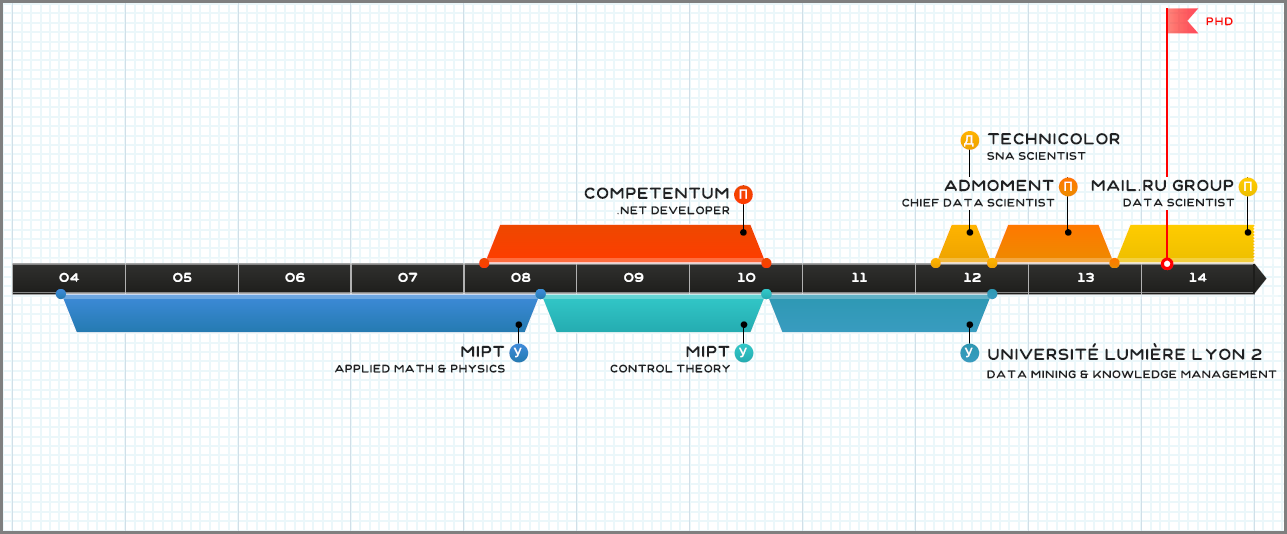
\includegraphics[scale=0.325]{images/timeline.png}
\end{center}

\begin{footnotesize}
e-mail: \href{mailto:n.anokhin@corp.mail.ru}{n.anokhin@corp.mail.ru} \\
тел.: +7 (903) 111-44-60
\end{footnotesize}

\end{frame}

\begin{frame}{План лекции}
\tableofcontents
\end{frame}

% =======================
\section{Структура курса}
% =======================

\begin{frame}{Структура курса}

{\small
Модуль 1
\begin{enumerate}
\item \underline{Задачи Data Mining (Николай Анохин)}
\item Задача кластеризации и EM-алгоритм (Николай Анохин)
\item Различные алгоритмы кластеризации (Николай Анохин){\color{red}$^{H}$}
\item Задача классификации (Николай Анохин)
\item Naive Bayes (Николай Анохин)
\item Линейные модели (Николай Анохин)
\item Метод опорных векторов (Николай Анохин){\color{red}$^{HP}$}
\end{enumerate}

Модуль 2
\begin{enumerate}
\item Снижение размерности пространства (Владимир Гулин)
\item Алгоритмические композиции 1 (Владимир Гулин)
\item Алгоритмические композиции 2 (Владимир Гулин){\color{red}$^{H}$}
\item Нейросети, обучение с учителем (Павел Нестеров){\color{red}$^{H}$}
\item Нейросети, обучение без учителя (Павел Нестеров)
\item Нейросети, глубокие сети (Павел Нестеров)
\end{enumerate}
}

\end{frame}

\begin{frame}{Контроль знаний}

\begin{block}{ДЗ}
4 домашних задания на 6-8 часов самостоятельной работы каждое (4x15 баллов)
\end{block}

\begin{center}
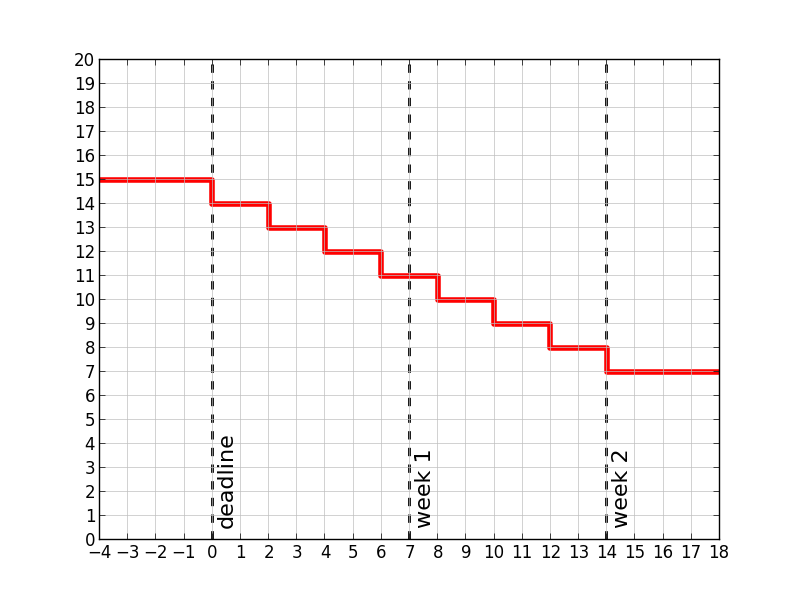
\includegraphics[scale=0.28]{images/hw.png}
\end{center}

\begin{alertblock}{Экзамен}
Презентация и защита семестрового проекта \\ (40 баллов)
\end{alertblock}

\end{frame}

\begin{frame}{Правила}

\begin{itemize}
\item[+] Можно задавать вопросы по ходу лекции
\item[+] Можно входить и выходить, не мешая коллегам
\item[---] Нельзя нарушать порядок в аудитории
\item[---] Нельзя разговаривать по телефону
\item Общение с преподавателем на ``Вы''
\end{itemize}

Ваши правила?

\end{frame}

% =======================
\section{Что такое Data Mining}
% =======================

\begin{frame}{DM как KDD}

\begin{block}{Data Mining}
Процесс извлечения знаний из различных источников данных, таких как базы данных, текст, картинки, видео и т.д. Полученные знания должны быть {\it достоверными}, {\it полезными} и {\it интерпретируемыми}.
\end{block}

\end{frame}

\begin{frame}{DM как моделирование}

\begin{block}{Data Mining}
Процесс построения модели, хорошо описывающей закономерности, которые порождают данные.
\end{block}

\vspace{1em}
Подходы к построению моделей
\begin{itemize}
\item[\color{green}\ding{52}] cтатистический
\item[\color{green}\ding{52}] на основании машинного обучения
\item[\color{red}\ding{54}] вычислительный
\end{itemize}

\end{frame}

\begin{frame}{DM и DS}

\begin{block}{Data Scientist}
Person who is better at statistics than any software engineer and better at software engineering than any statistician \\ (J. Wills, Data Scientist at Cloudera Inc.)
\end{block}

\vspace{1em}
Data-
\begin{itemize}
\item[\color{red}\ding{54}] -architecture
\item[\color{red}\ding{54}] -acquisition
\item[\color{green}\ding{52}] -analysis
\item[\color{red}\ding{54}] -archiving
\end{itemize}

\end{frame}

\begin{frame}{Success stories}

\begin{figure}
        \centering
        \begin{subfigure}[b]{0.45\textwidth}
                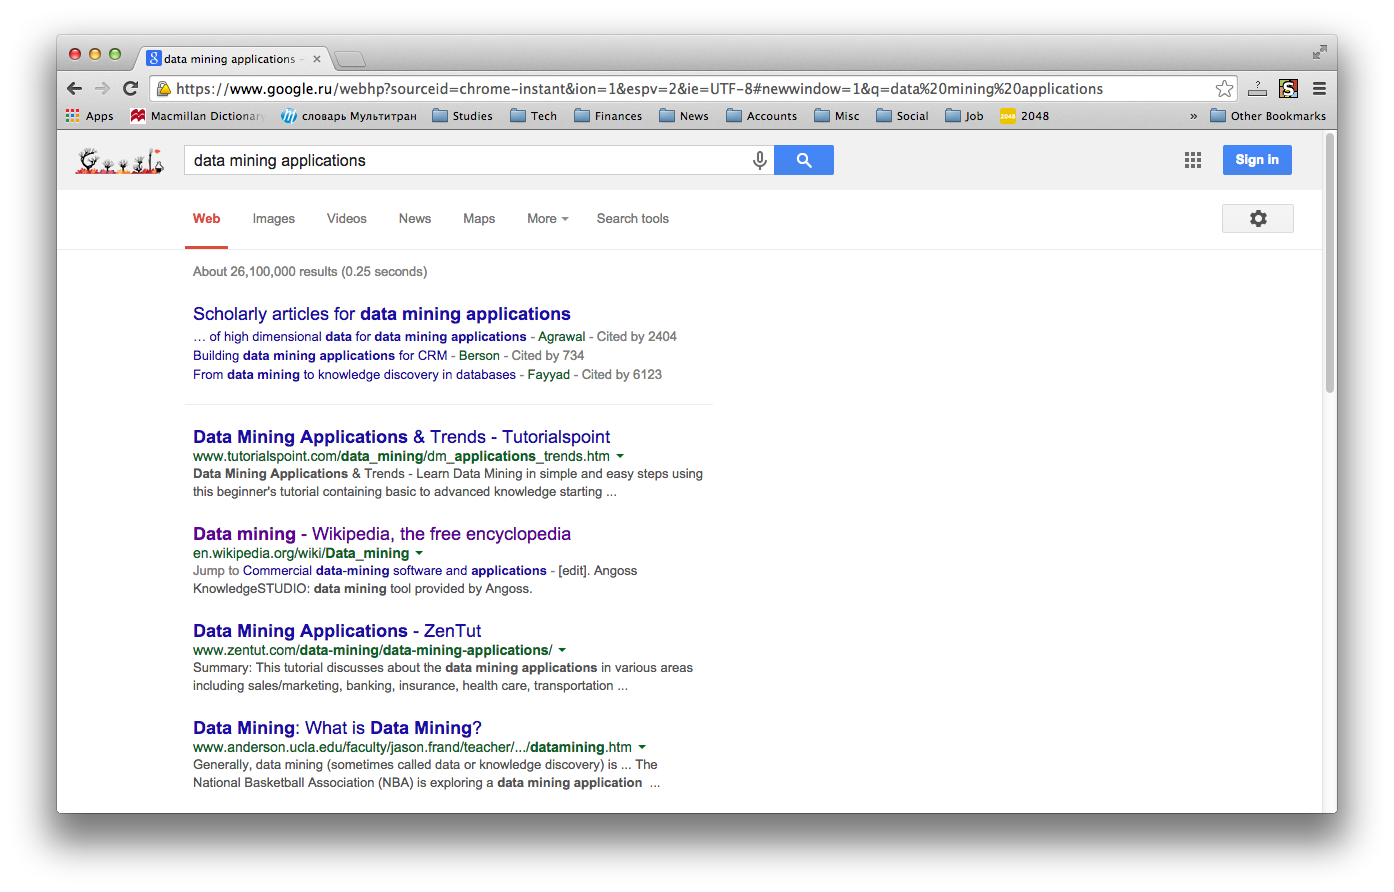
\includegraphics[width=\textwidth]{images/google.png}
                \caption{Google}                
        \end{subfigure}%        
        \begin{subfigure}[b]{0.45\textwidth}
                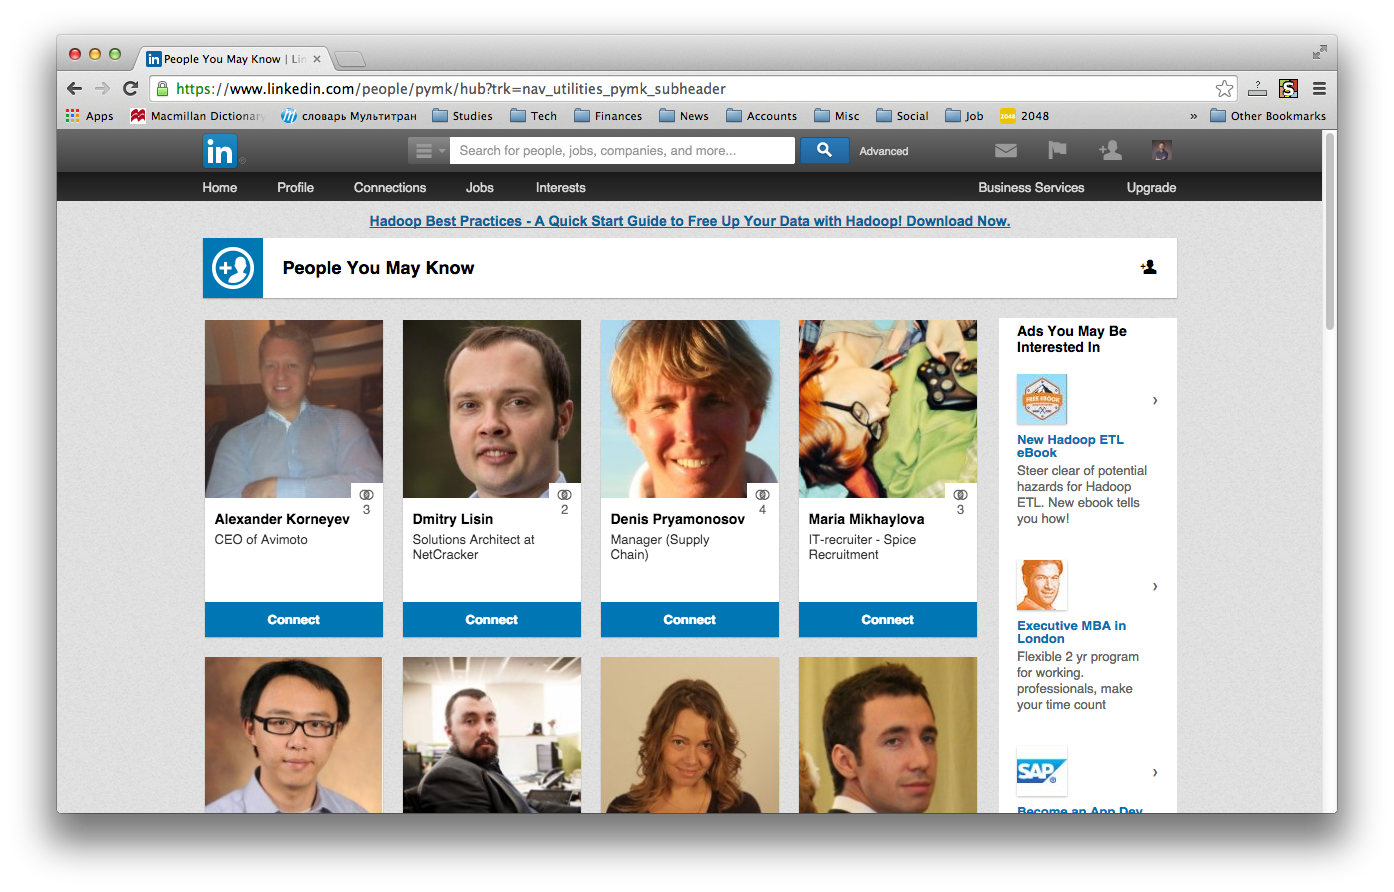
\includegraphics[width=\textwidth]{images/linkedin.png}
                \caption{LinkedIn}     
        \end{subfigure}
        
        \begin{subfigure}[b]{0.45\textwidth}
                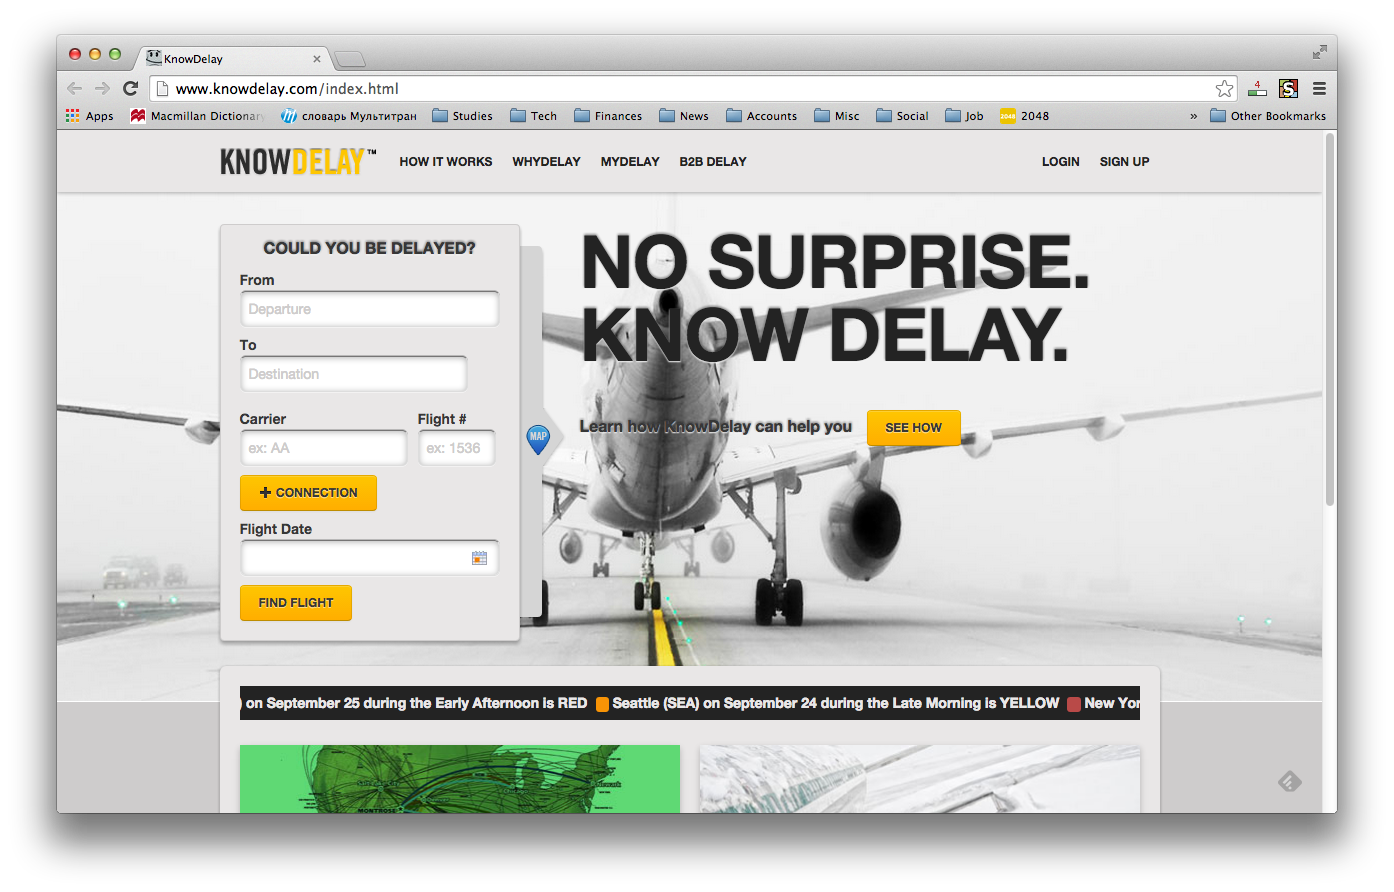
\includegraphics[width=\textwidth]{images/delay.png}
                \caption{KnowDelay}                
        \end{subfigure}%        
        \begin{subfigure}[b]{0.45\textwidth}
                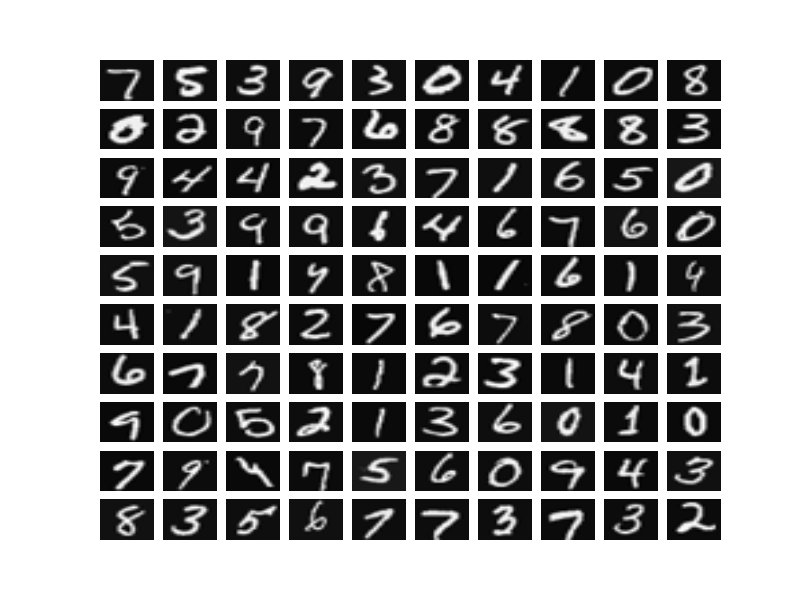
\includegraphics[width=0.9\textwidth]{images/digits.png}
                \caption{Handwritten digits}
        \end{subfigure}
\end{figure}

\end{frame}

\begin{frame}{Fail (Программа TIA)}

\begin{itemize}
\item Наблюдаем $10^9$ человек
\item Человек в среднем посещает отель раз в $100$ дней
\item Есть $10^5$ отелей на $100$ человек каждый
\item Проверим посещения за $1000$ дней 
\end{itemize}

Вероятность для конкретной пары встретиться в отеле в конкретный день:
\[
p_1 = \left(\frac{1}{100}\right)^2 \cdot 10^{-5} = 10^{-9}
\]
Всего пар людей
\[
n_{pp} = C^{10^9}_2 \approx \frac{(10^9)^2}{2} = 5 \cdot 10^{17}
\]
а пар дней
\[
n_{pd} = C^{10^3}_2 \approx \frac{(10^3)^2}{2} = 5 \cdot 10^{5}
\]
Ожидаемое количество ``подозрительных'' встреч в отелях
\[
N = p_1^2 n_{pp} n_{pd} = 250000 >> 10
\]

\end{frame}

\begin{frame}{Принцип Бонферрони}

Вычислить количество рассматриваемых событий при предположении их полной случайности. Если это количество намного превосходит количество событий, о котором идет речь в задаче, полученные результаты нельзя будет считать достоверными.

\end{frame}

% =======================
\section{Унификация процесса Data Mining}
% =======================

\begin{frame}{Cross Industry Standard Process for Data Mining}

\begin{columns}[C]
    \begin{column}{.5\textwidth}
    	CRISP-DM   	
    	\begin{itemize}
    		\item SPSS 
    		\item Teradata 
   			\item Daimler AG 
    		\item NCR Corporation 
    		\item OHRA
    		\item IBM
		\end{itemize}
		
		Другие процессы: KDD, SEMMA 	
    \end{column}
    %   
    \begin{column}{.5\textwidth}
    \vspace{-0em}
	\begin{center}
   		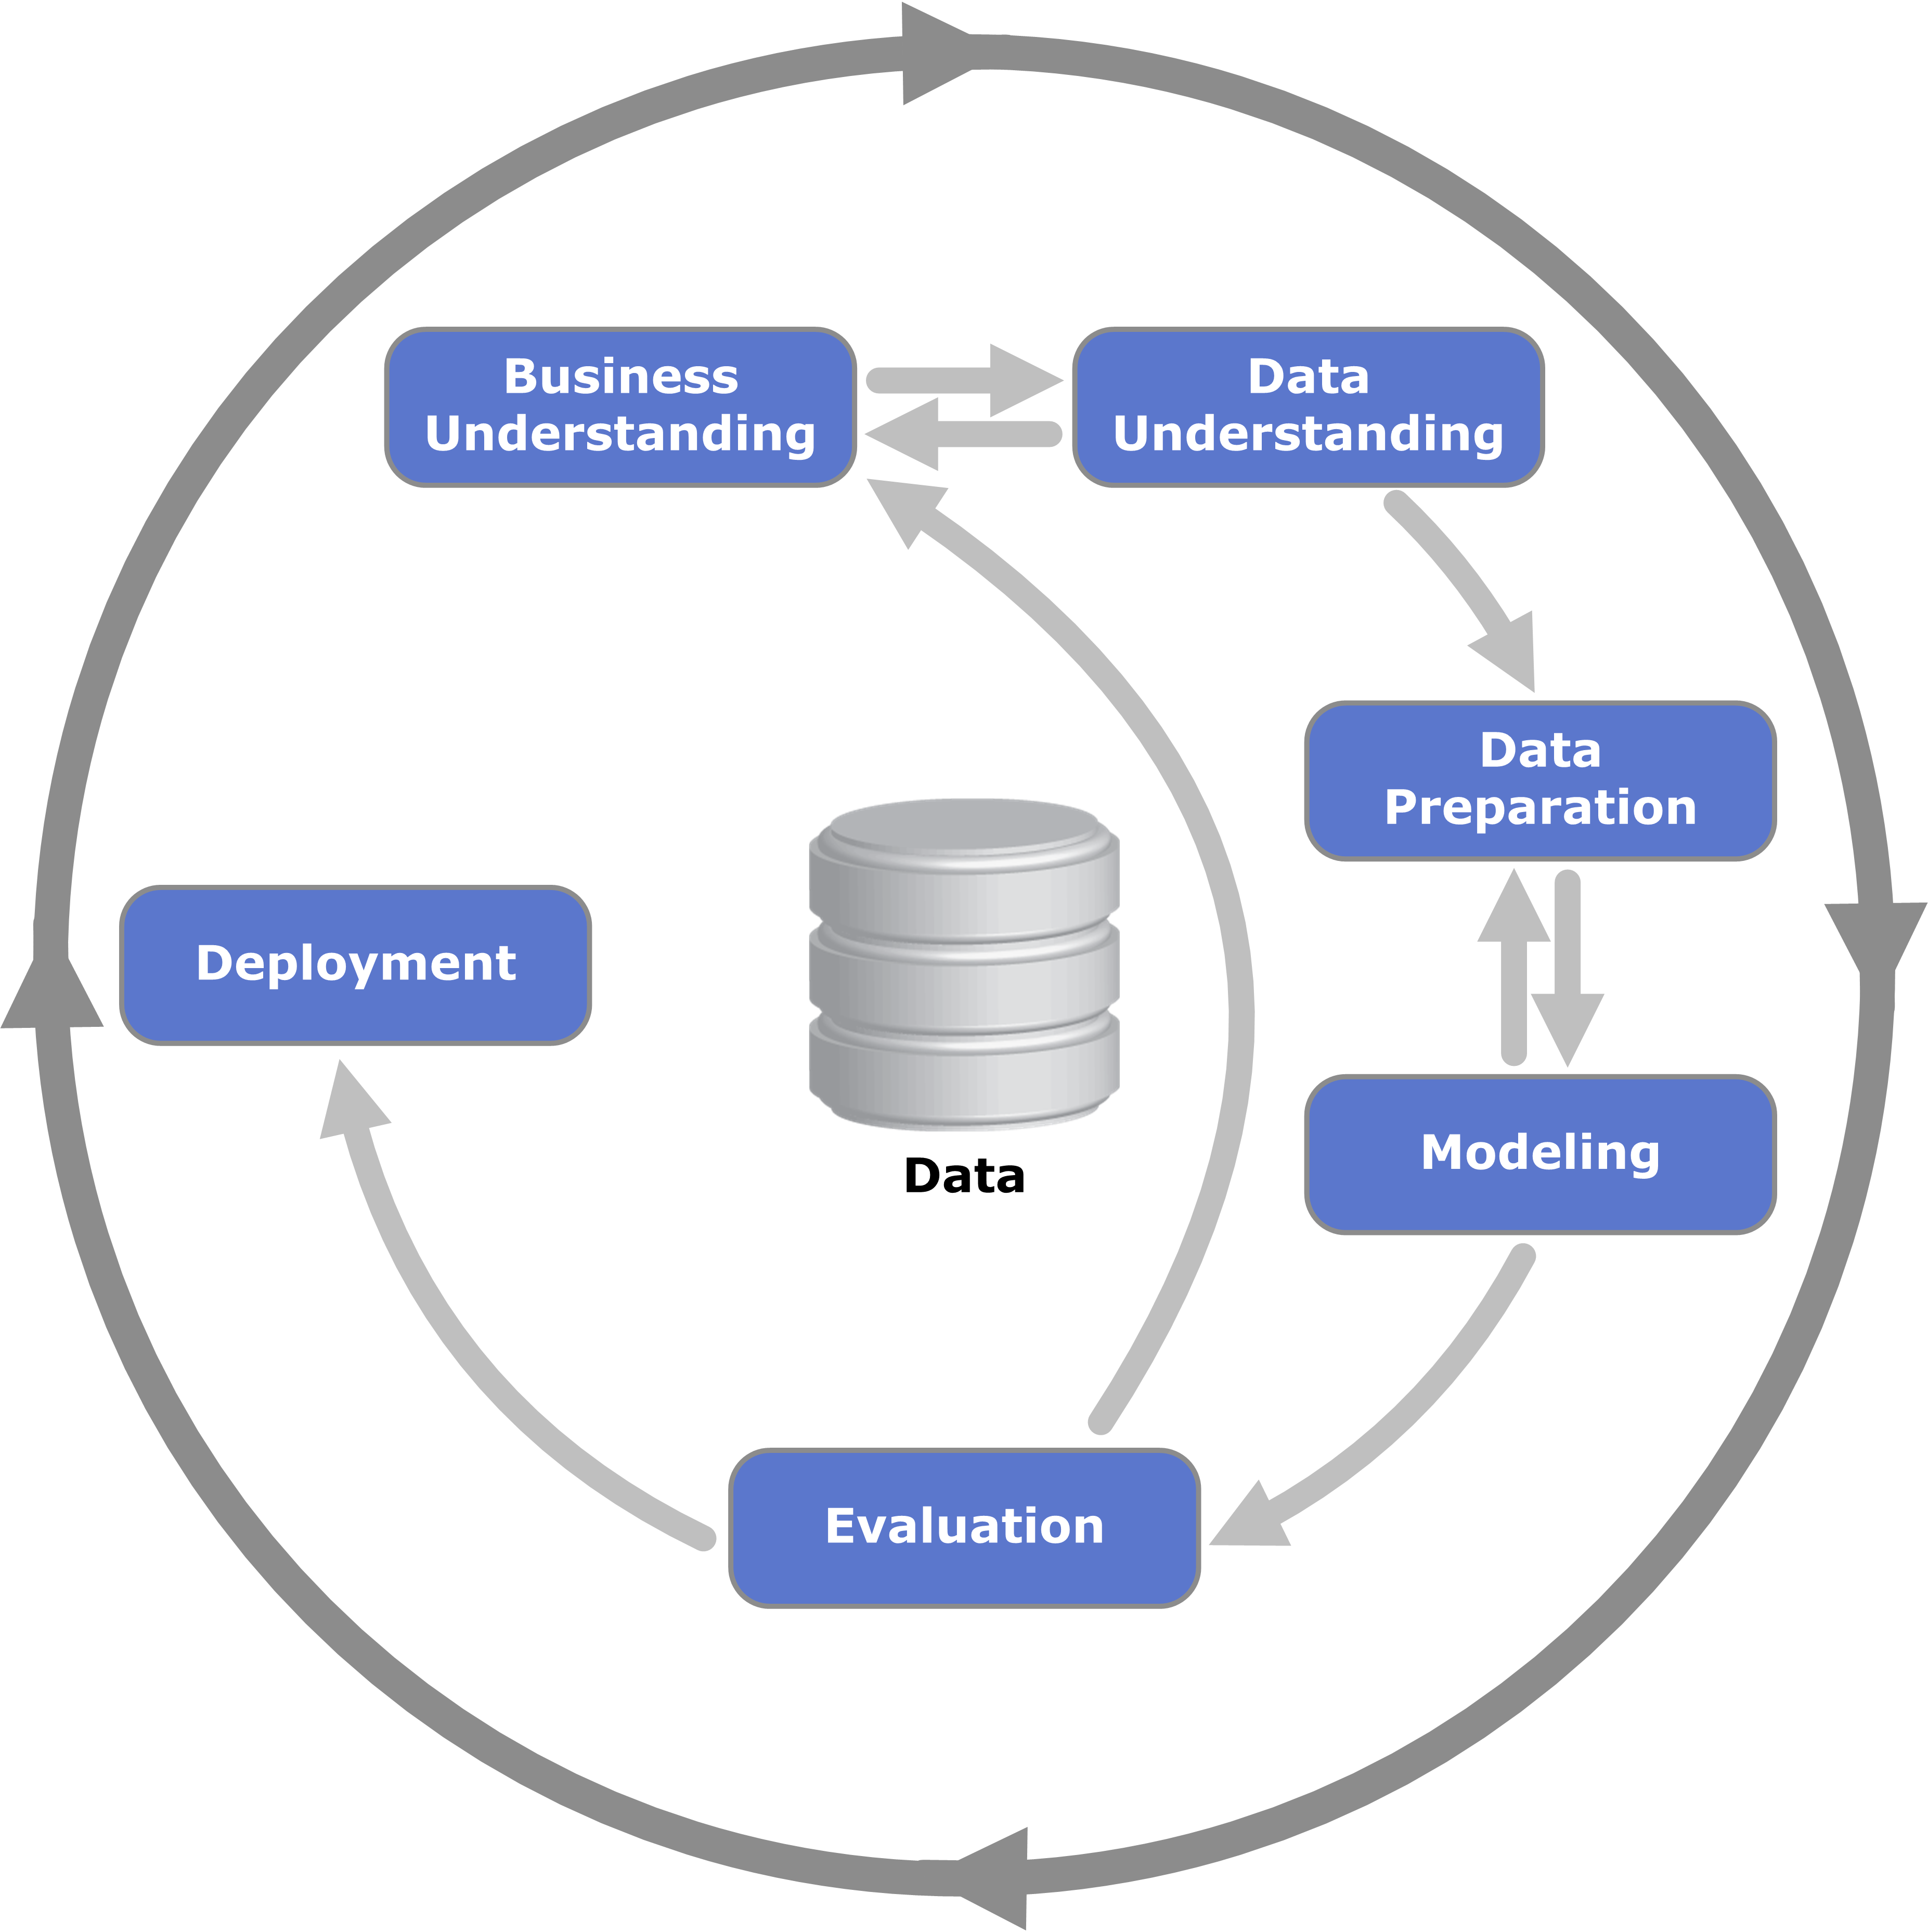
\includegraphics[width=\textwidth]{images/crisp.png}
    \end{center}
    \end{column}
  \end{columns}

\end{frame}

\begin{frame}{}

\begin{columns}[C]
    \begin{column}{.5\textwidth}
    {\it Задача:} на рыболовном предприятии автоматизировать сортировку улова
    \begin{figure}
        \centering
        \begin{subfigure}[b]{\textwidth}
                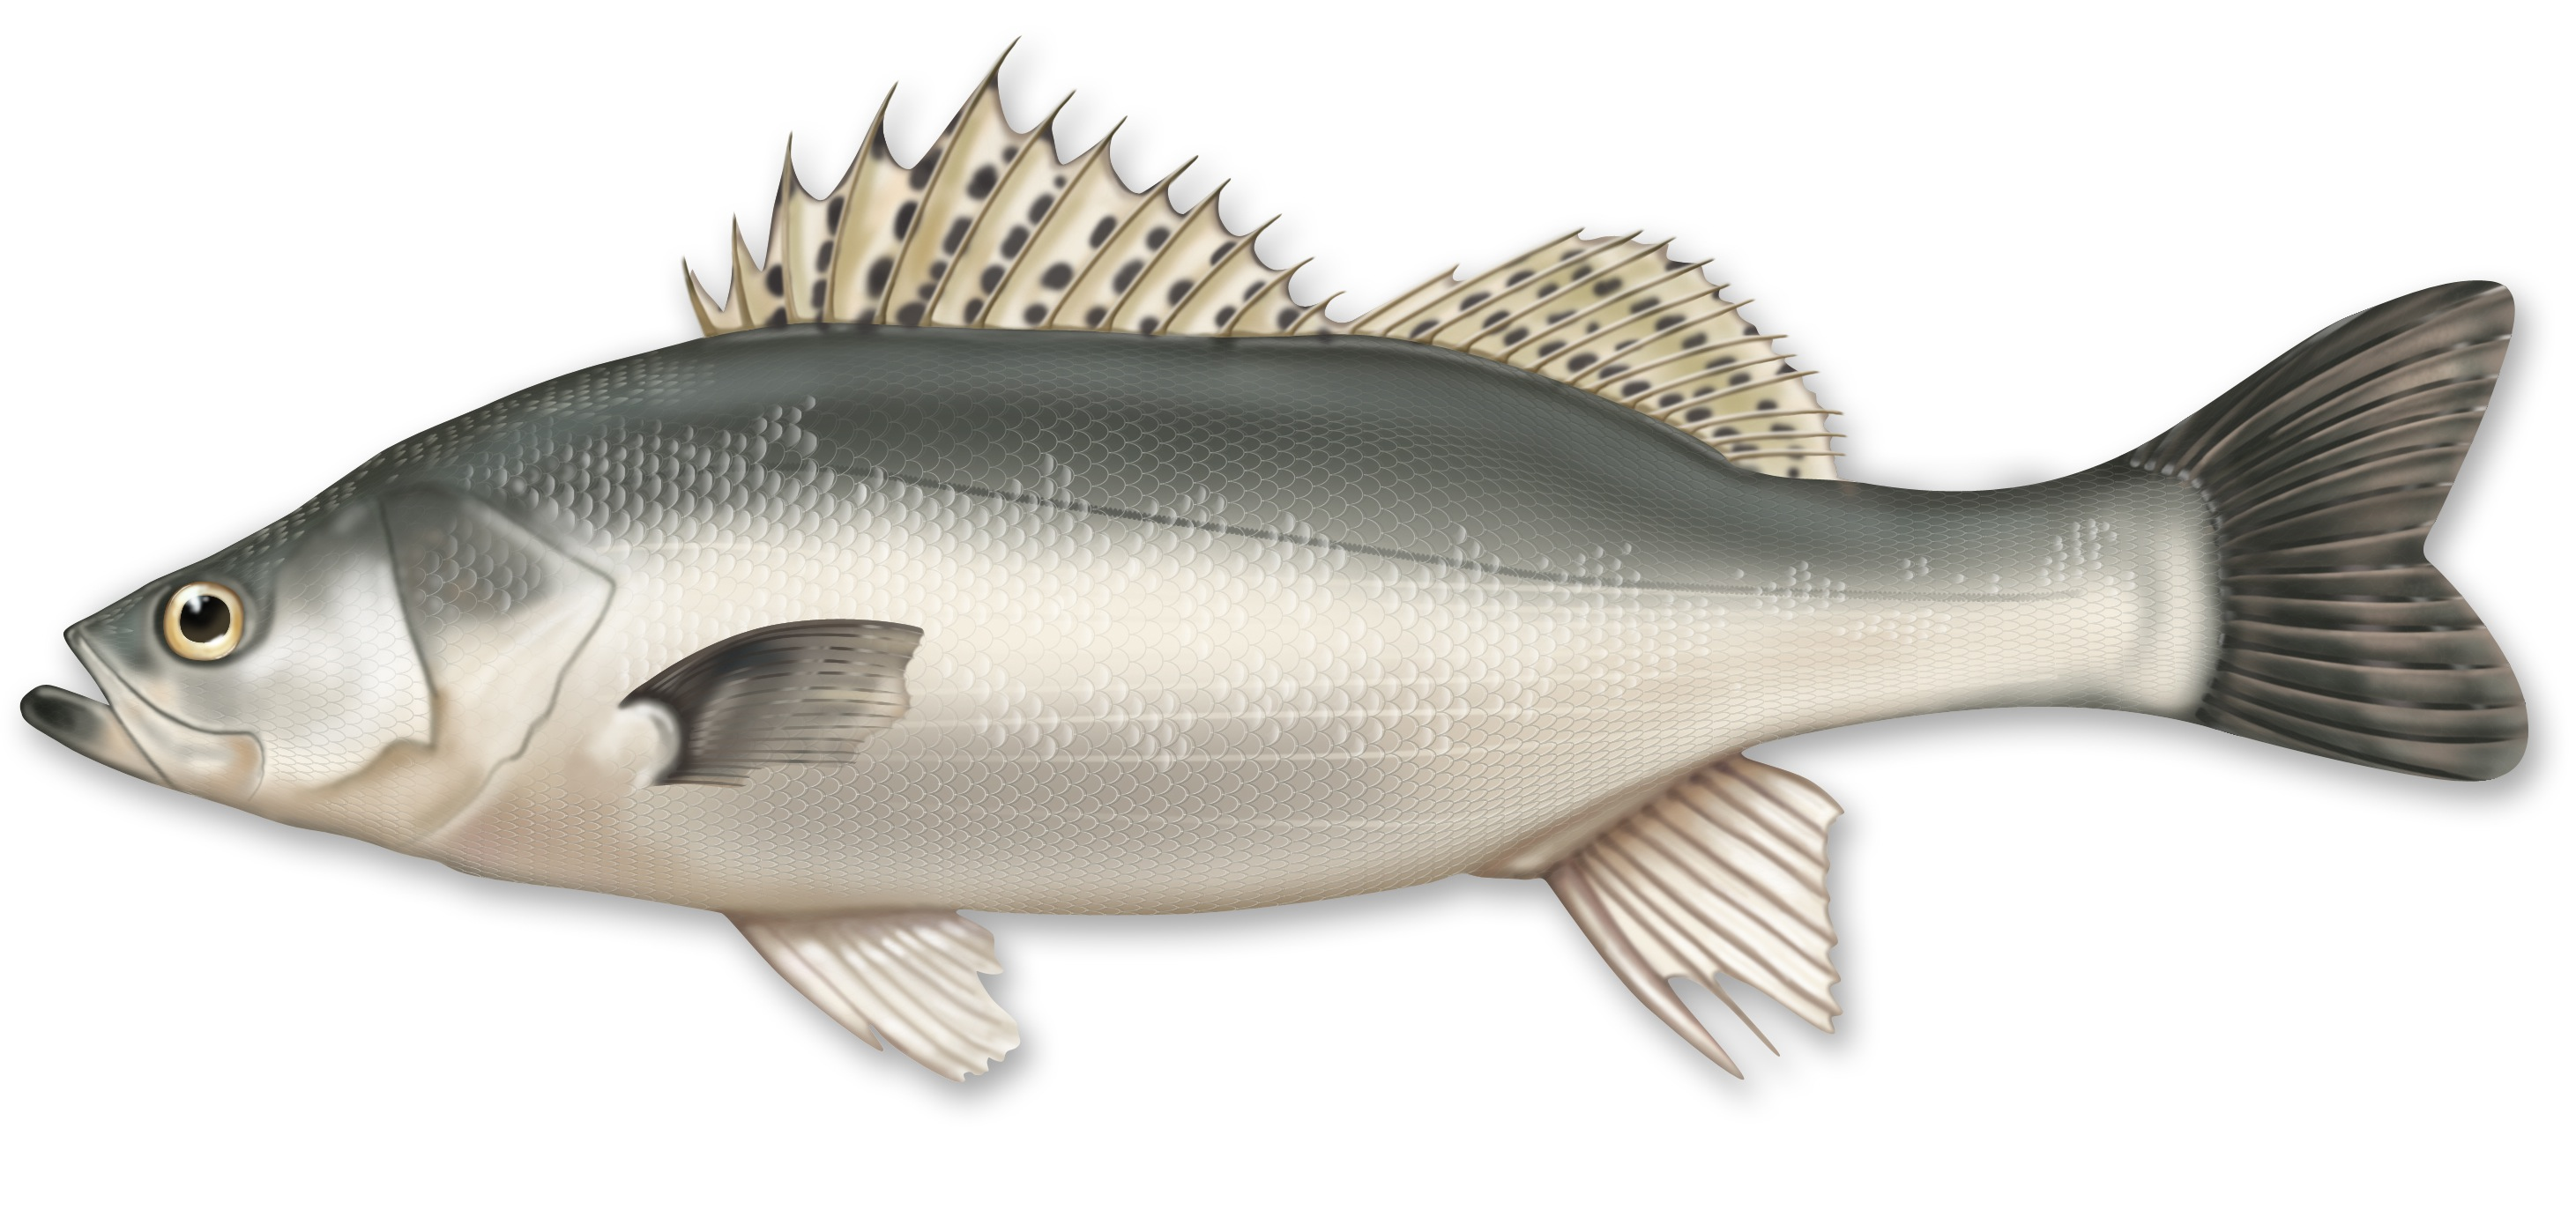
\includegraphics[width=0.9\textwidth]{images/seabass.jpg}
                \caption{Сибас}                
        \end{subfigure}
            
        \begin{subfigure}[b]{\textwidth}
                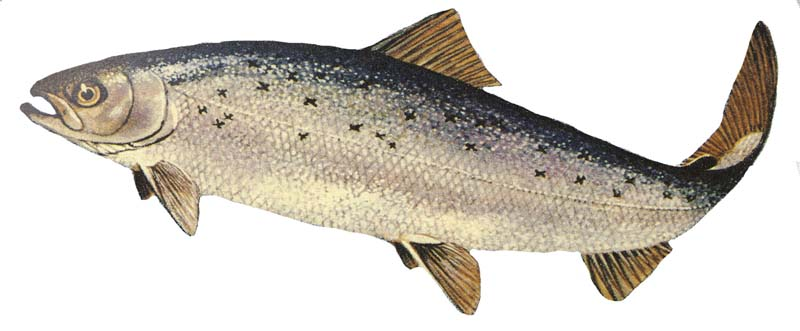
\includegraphics[width=0.9\textwidth]{images/salmon.jpg}
                \caption{Лосось}     
        \end{subfigure}
	\end{figure}    
    \end{column}
    %
    \begin{column}{.5\textwidth}
    \vspace{-0em}
	\begin{center}
   		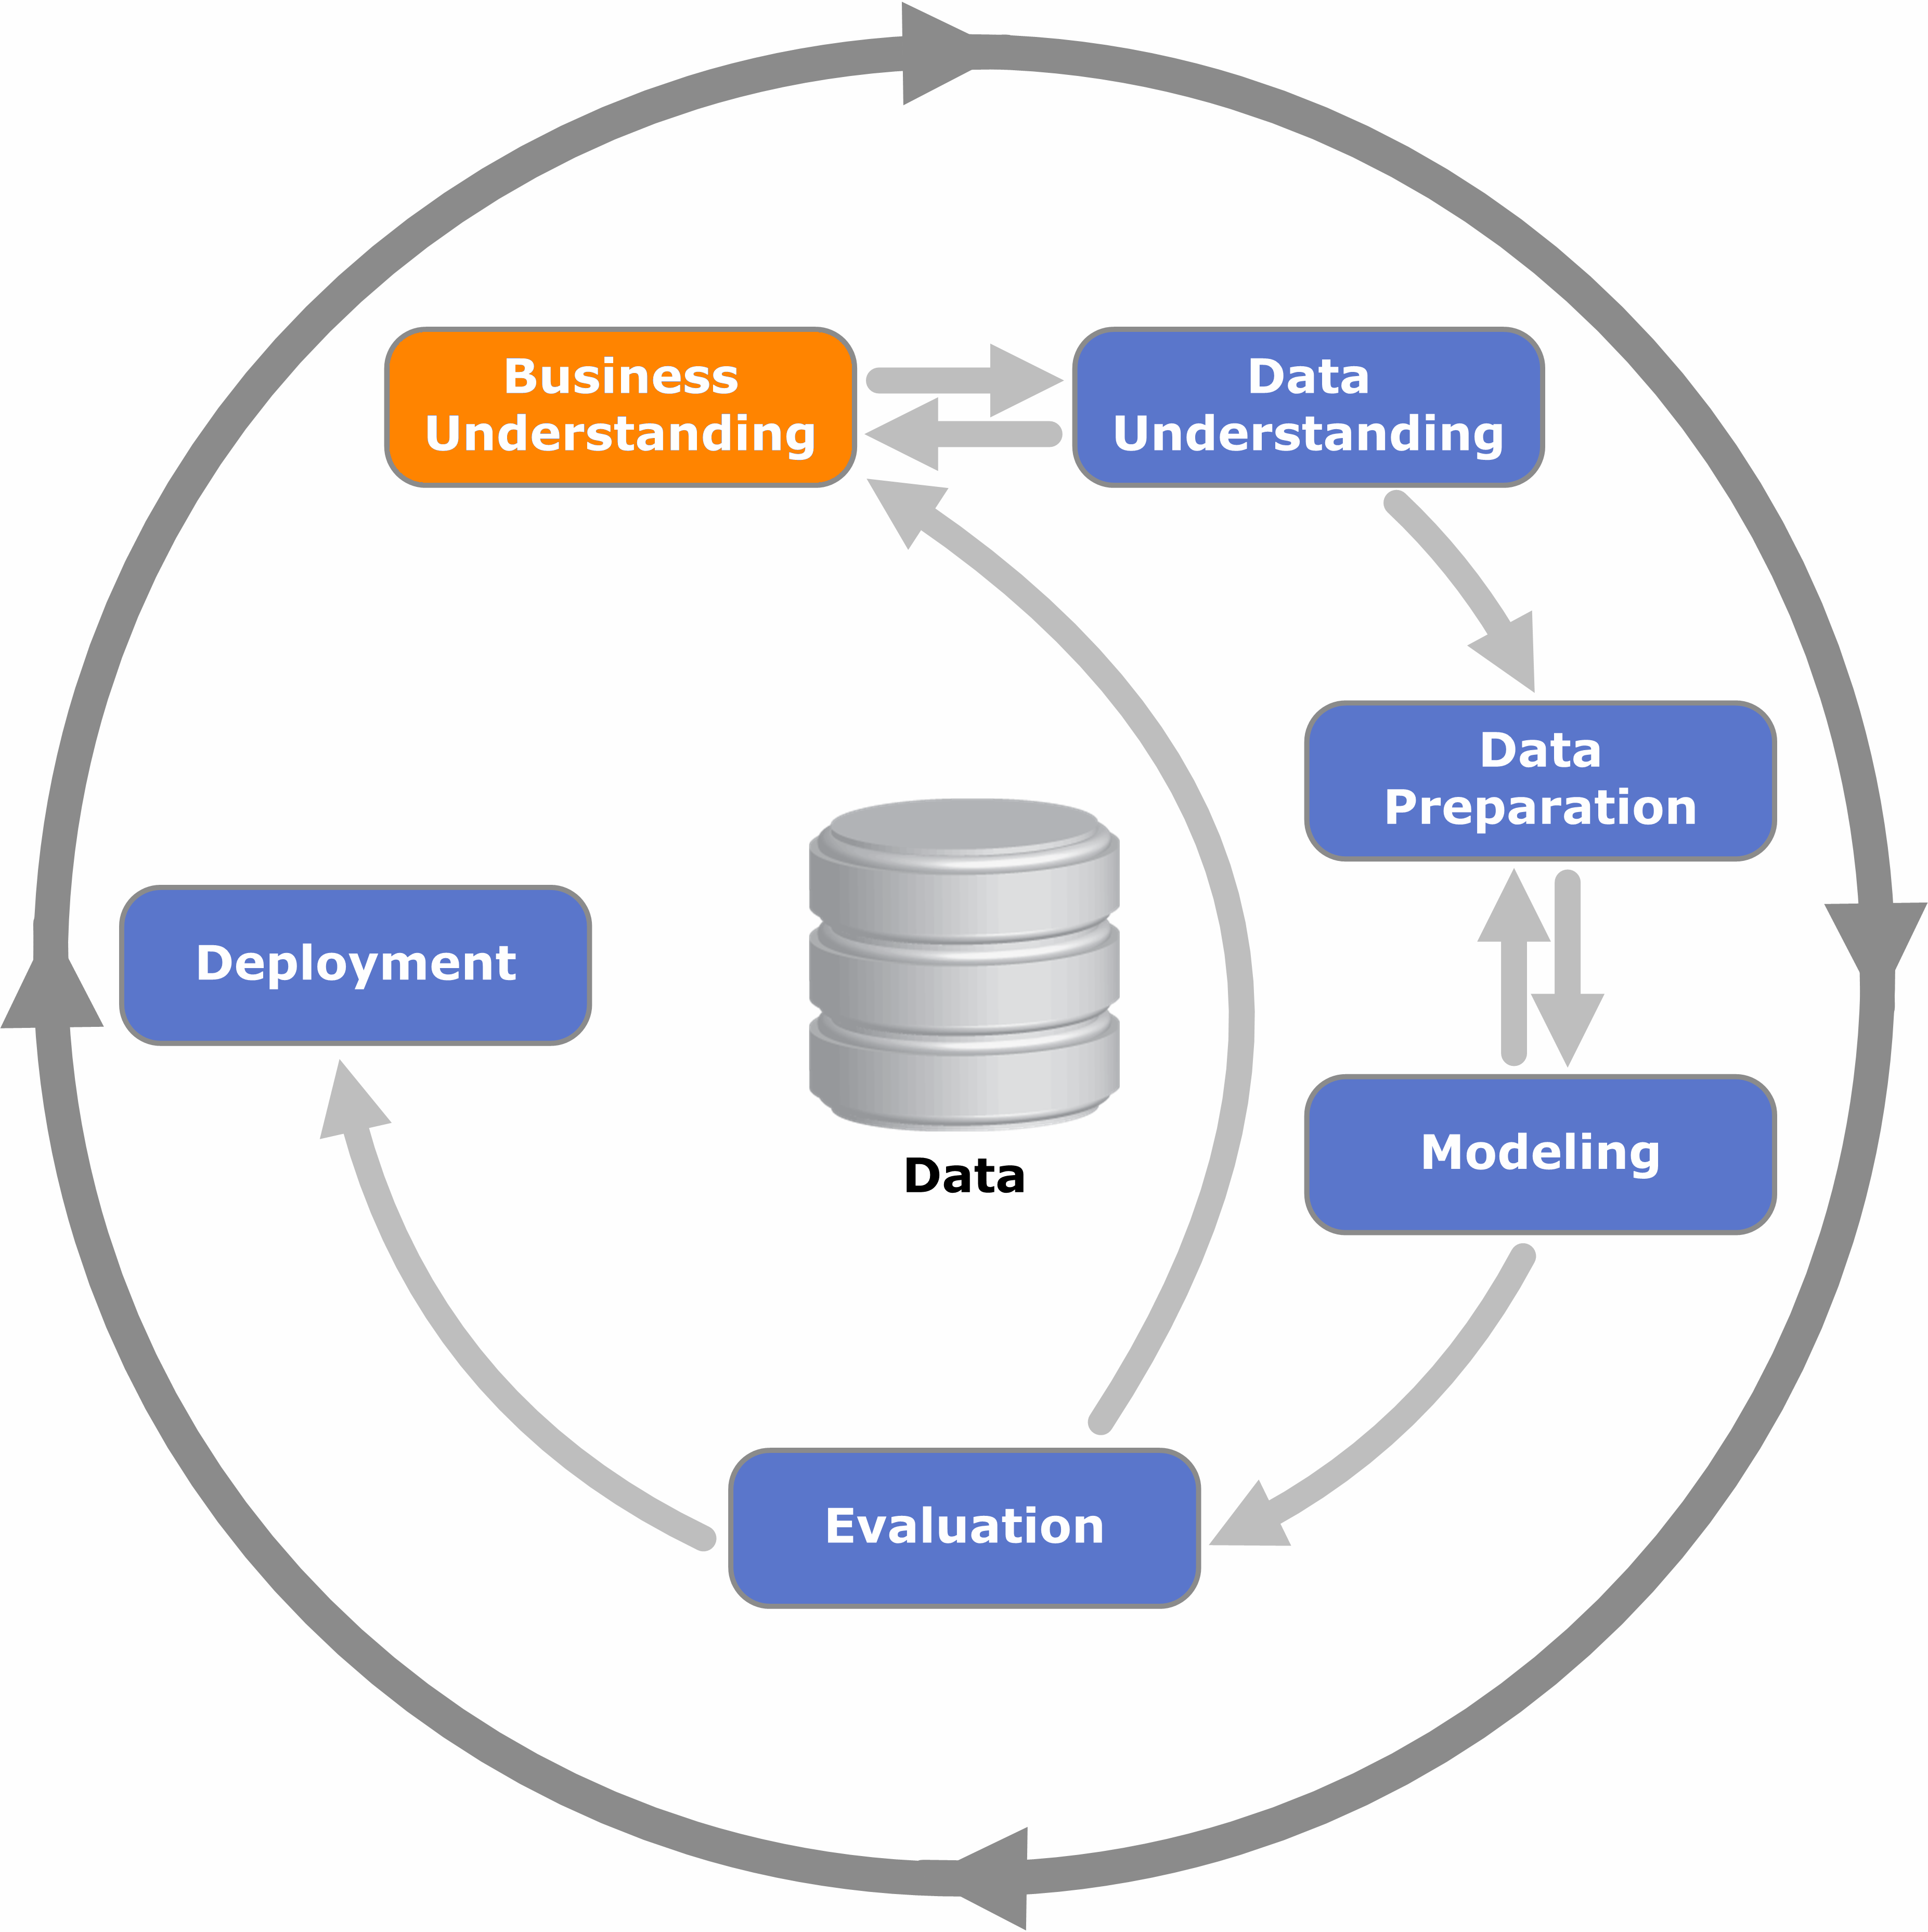
\includegraphics[width=\textwidth]{images/crisp-bu.png}
    \end{center}
    \end{column}
  \end{columns}

\end{frame}

\begin{frame}{Признаки}

\begin{columns}[C]
    \begin{column}{.5\textwidth}
    $\mathcal{D}$ -- множество объектов (data set) \\
    $d \in \mathcal{D}$ -- обучающий объект \\
    $\phi_j: D \rightarrow F_j$ -- признак
    
    \vspace{1em}
    Виды признаков
    \begin{itemize}
    \item Бинарные/Binary \\ $F_j = \{true, false\}$
	\item Номинальные/Categorical \\ $F_j$ -- конечно
	\item Порядковый/Ordinal \\ $F_j$ -- конечно, упорядочено
	\item Количественный/Numerical \\ $F_j = \mathbb{R}$
    \end{itemize}
    \vspace{1em}
    Представление $d_i$
    \[
    \mathbf{x}_i = (\phi_1(d_i), \ldots, \phi_n(d_i)) \in \mathcal{X}
    \]

    \end{column}
       
    \begin{column}{.5\textwidth}
    \vspace{-0em}
	\begin{center}
   		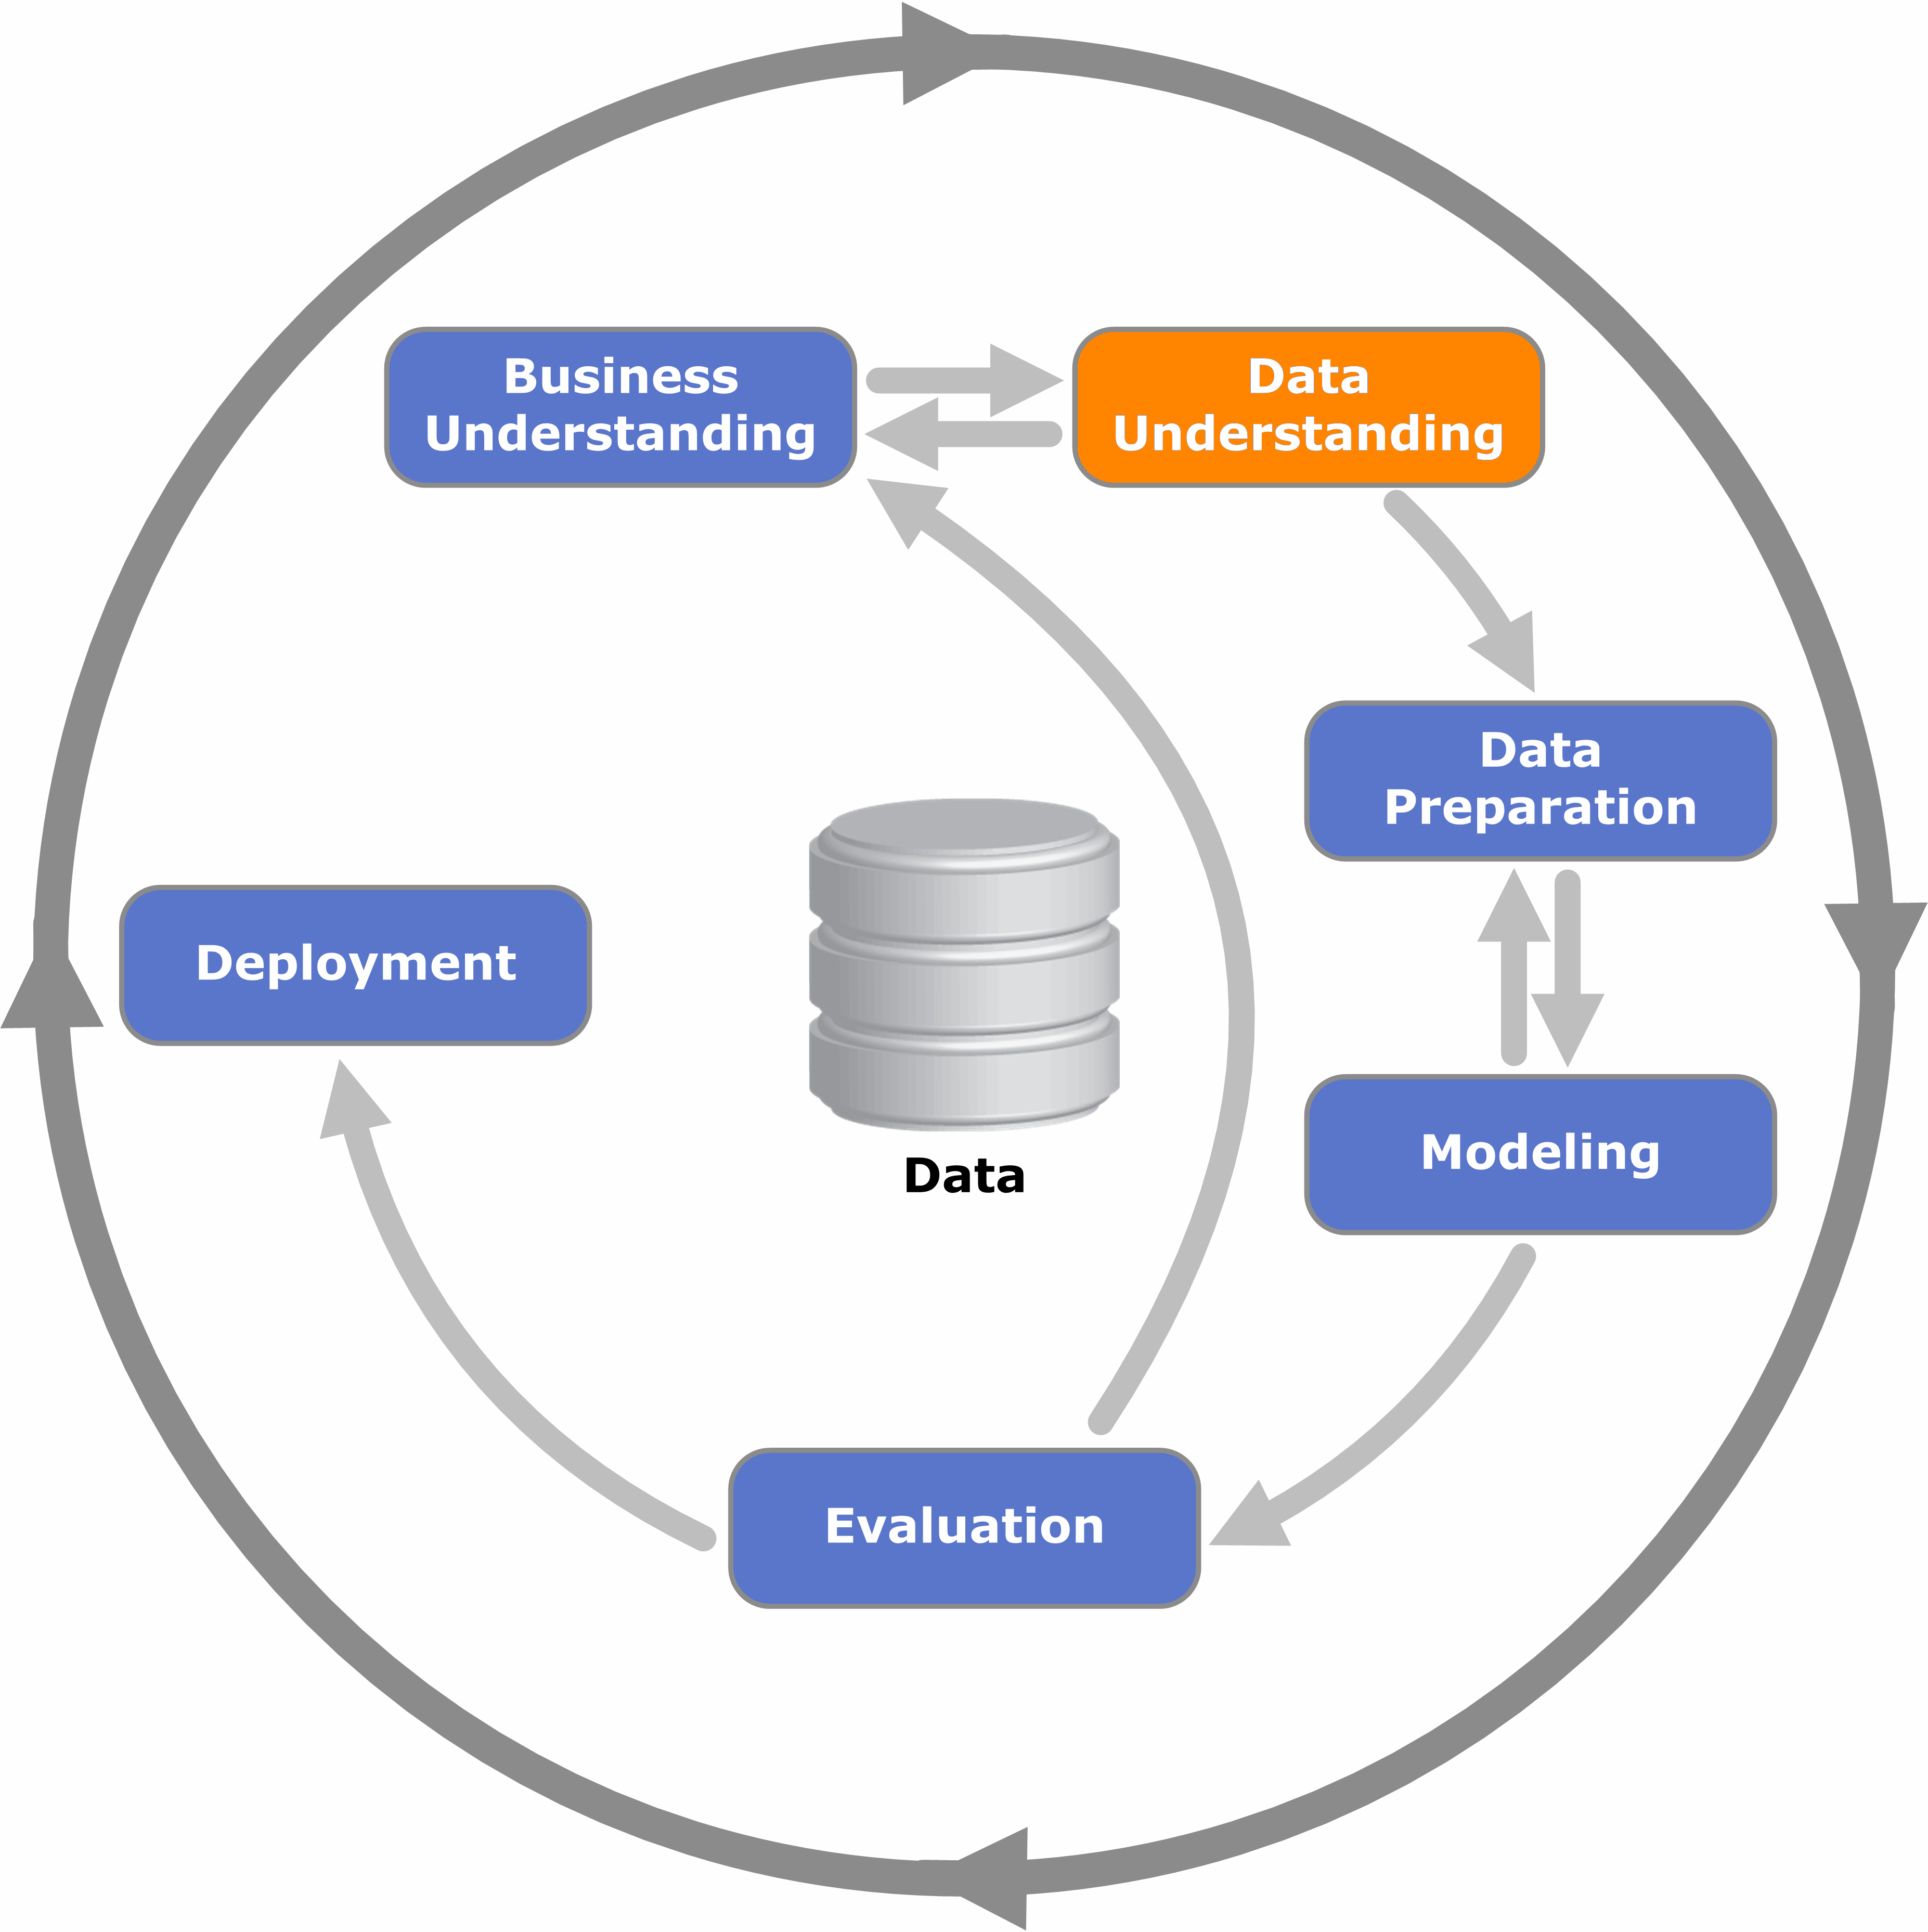
\includegraphics[width=\textwidth]{images/crisp-du.png}
    \end{center}
    \end{column}
  \end{columns}

\end{frame}

\begin{frame}{}

\begin{columns}[C]
    \begin{column}{.5\textwidth}
    \begin{itemize}
		\item Удаление шума
		\item Заполнение отсутствующих значений
		\item Трансформация факторов
		\item Выбор факторов
		\item Использование априорных знаний
	\end{itemize}
	\vspace{1em}
	В итоге:\\
	\[
	X = \begin{pmatrix}
	\mathbf{x_1} \\
	\ldots \\
	\mathbf{x_N} \\
	\end{pmatrix}, \;\; x_i \in \mathcal{X}
	\]
	\[
	Y = \begin{pmatrix}
	y_1 \\
	\ldots \\
	y_N \\
	\end{pmatrix}, \;\; y_i \in \mathcal{Y}
	\]
    \end{column}
       
    \begin{column}{.5\textwidth}
    \vspace{-0em}
	\begin{center}
   		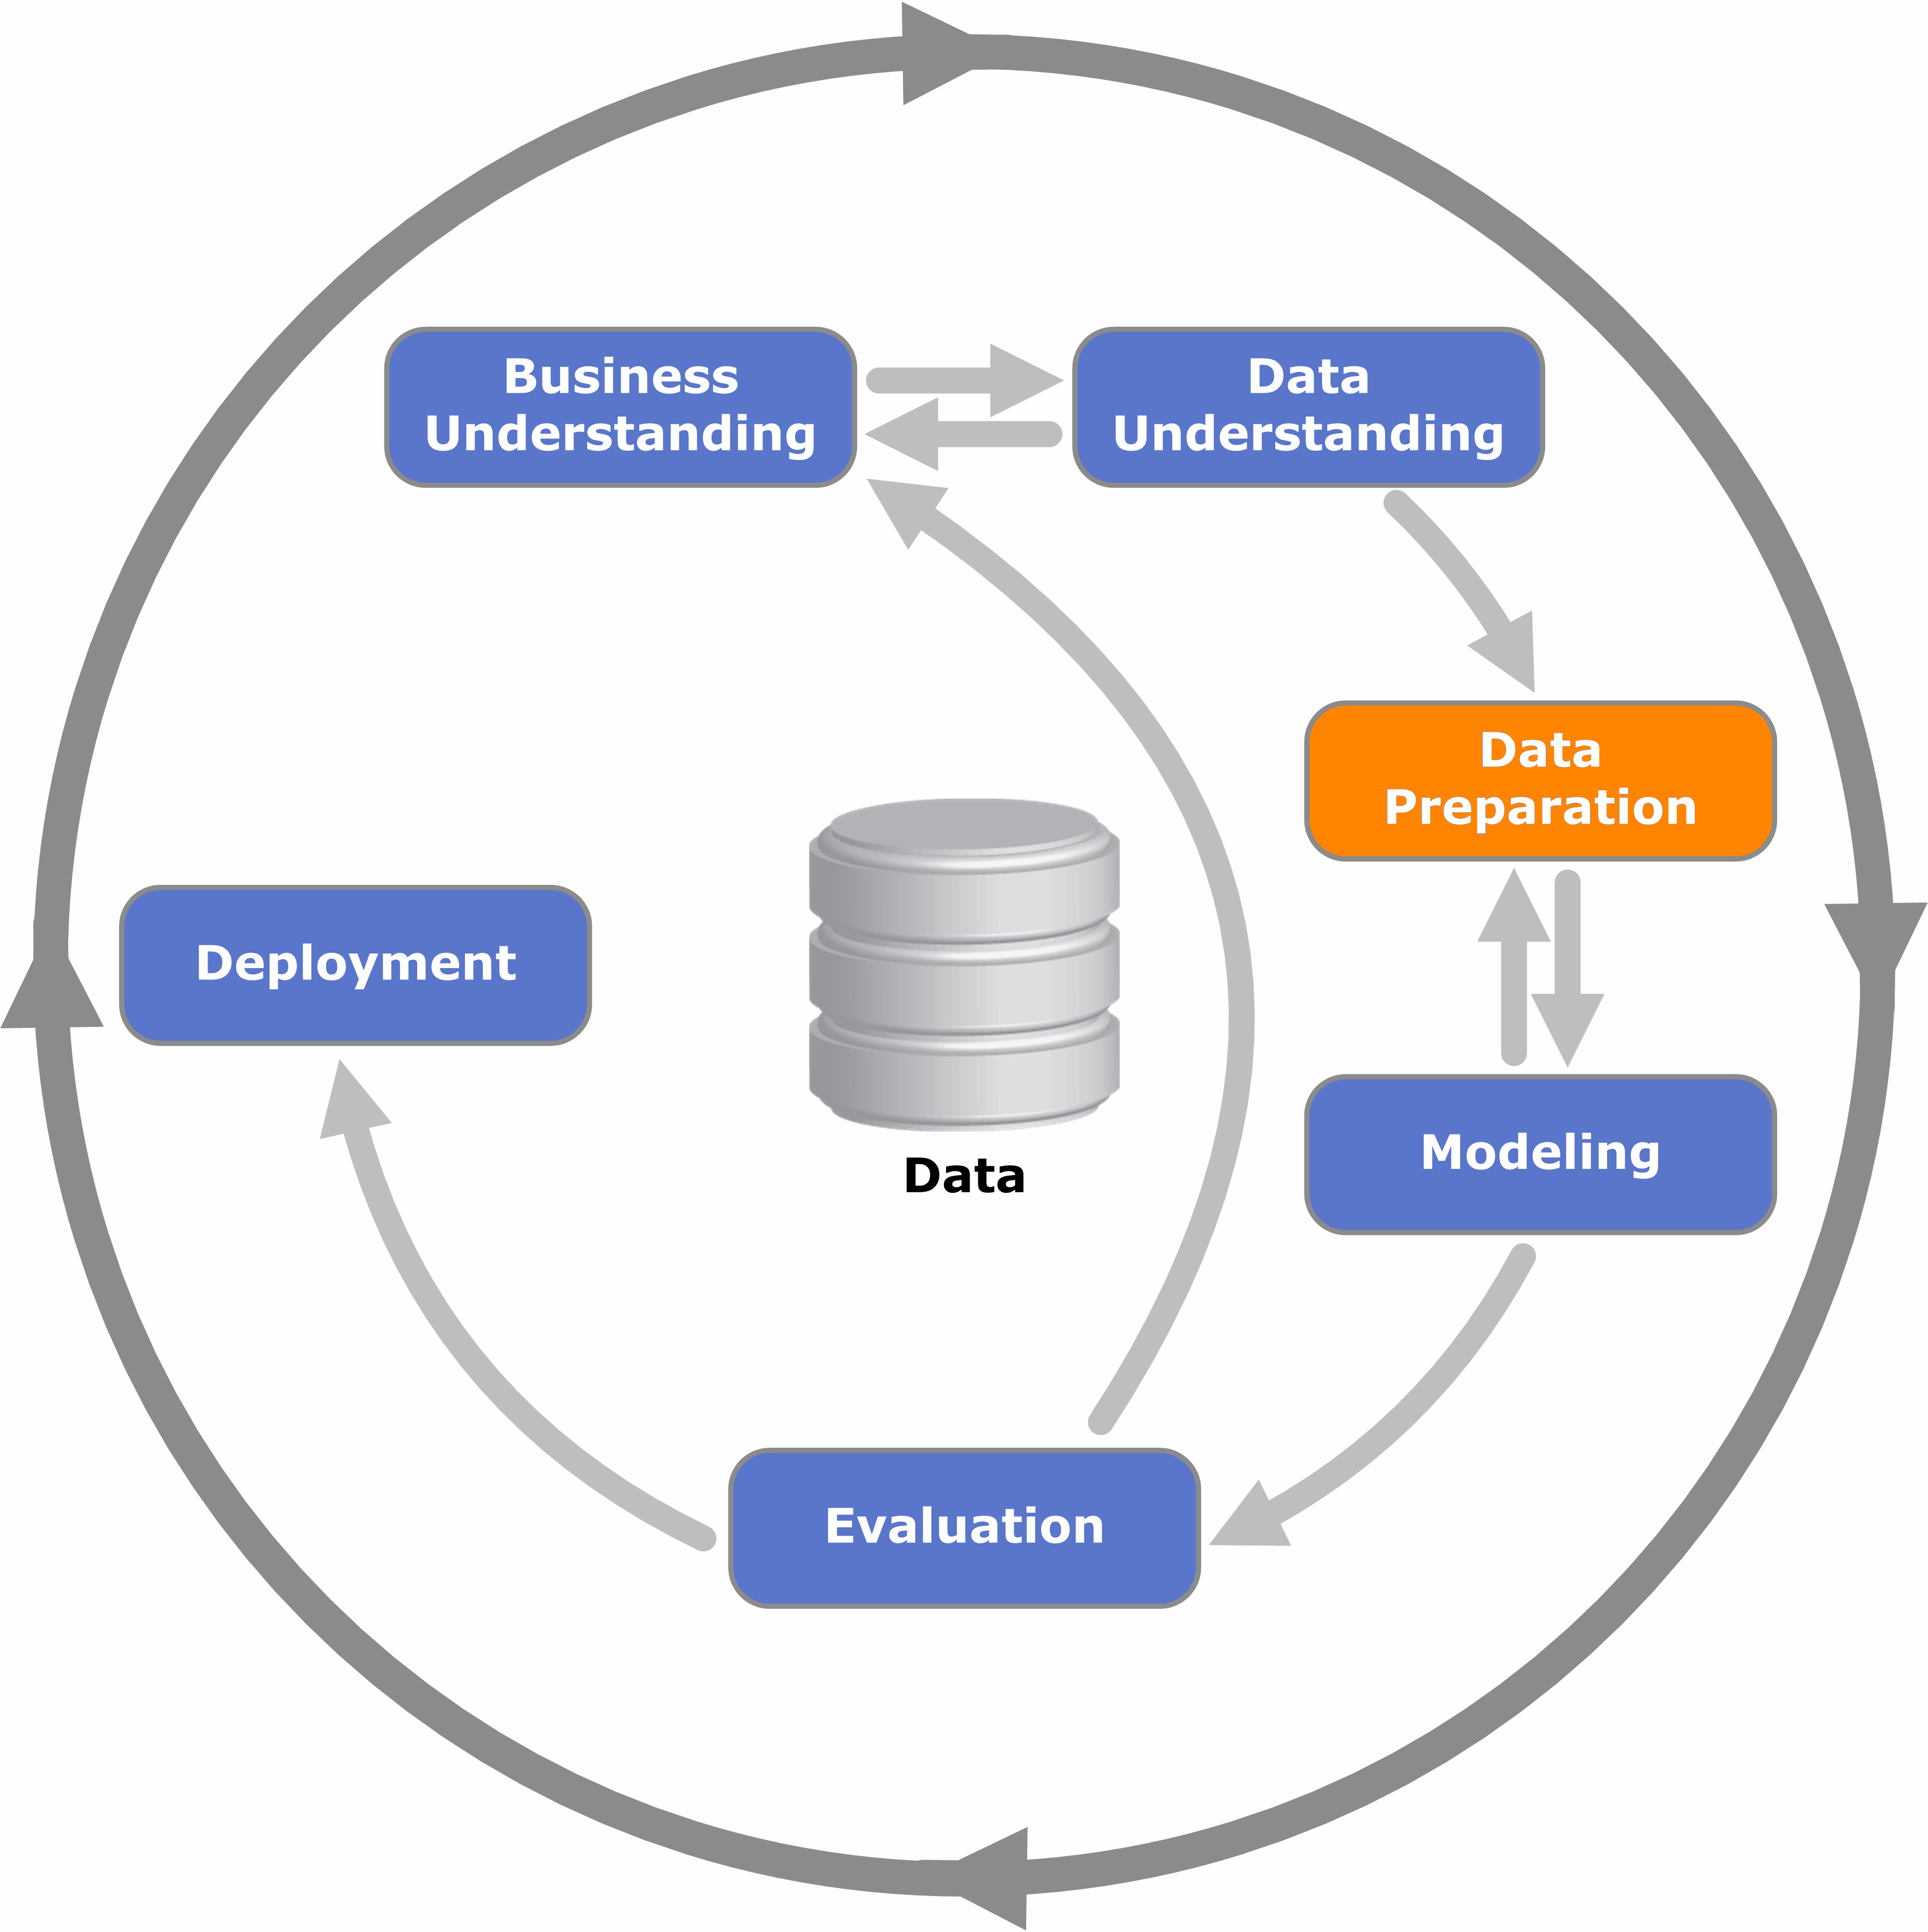
\includegraphics[width=\textwidth]{images/crisp-dp.png}
    \end{center}
    \end{column}
  \end{columns}

\end{frame}

\begin{frame}{}

\begin{columns}[C]
    \begin{column}{.5\textwidth}
    \begin{block}{Модель}
    семейство параметрических функций вида
    \[
    H = \{h(\mathbf{x}, \theta): \mathcal{X} \times \Theta \rightarrow \mathcal{Y} \}
    \]    
    \end{block}
    \begin{block}{Алгоритм обучения}
    выбор наилучших параметров $\theta^*$
    \[
    A(X, Y): (\mathcal{X} \times \mathcal{Y})^N \rightarrow \Theta
    \]    
    \end{block}
    В итоге:
    \[
    h^*(\mathbf{x}) = h(\mathbf{x}, \theta^*)
    \]
    		
    \end{column}
       
    \begin{column}{.5\textwidth}
    \vspace{-0em}
	\begin{center}
   		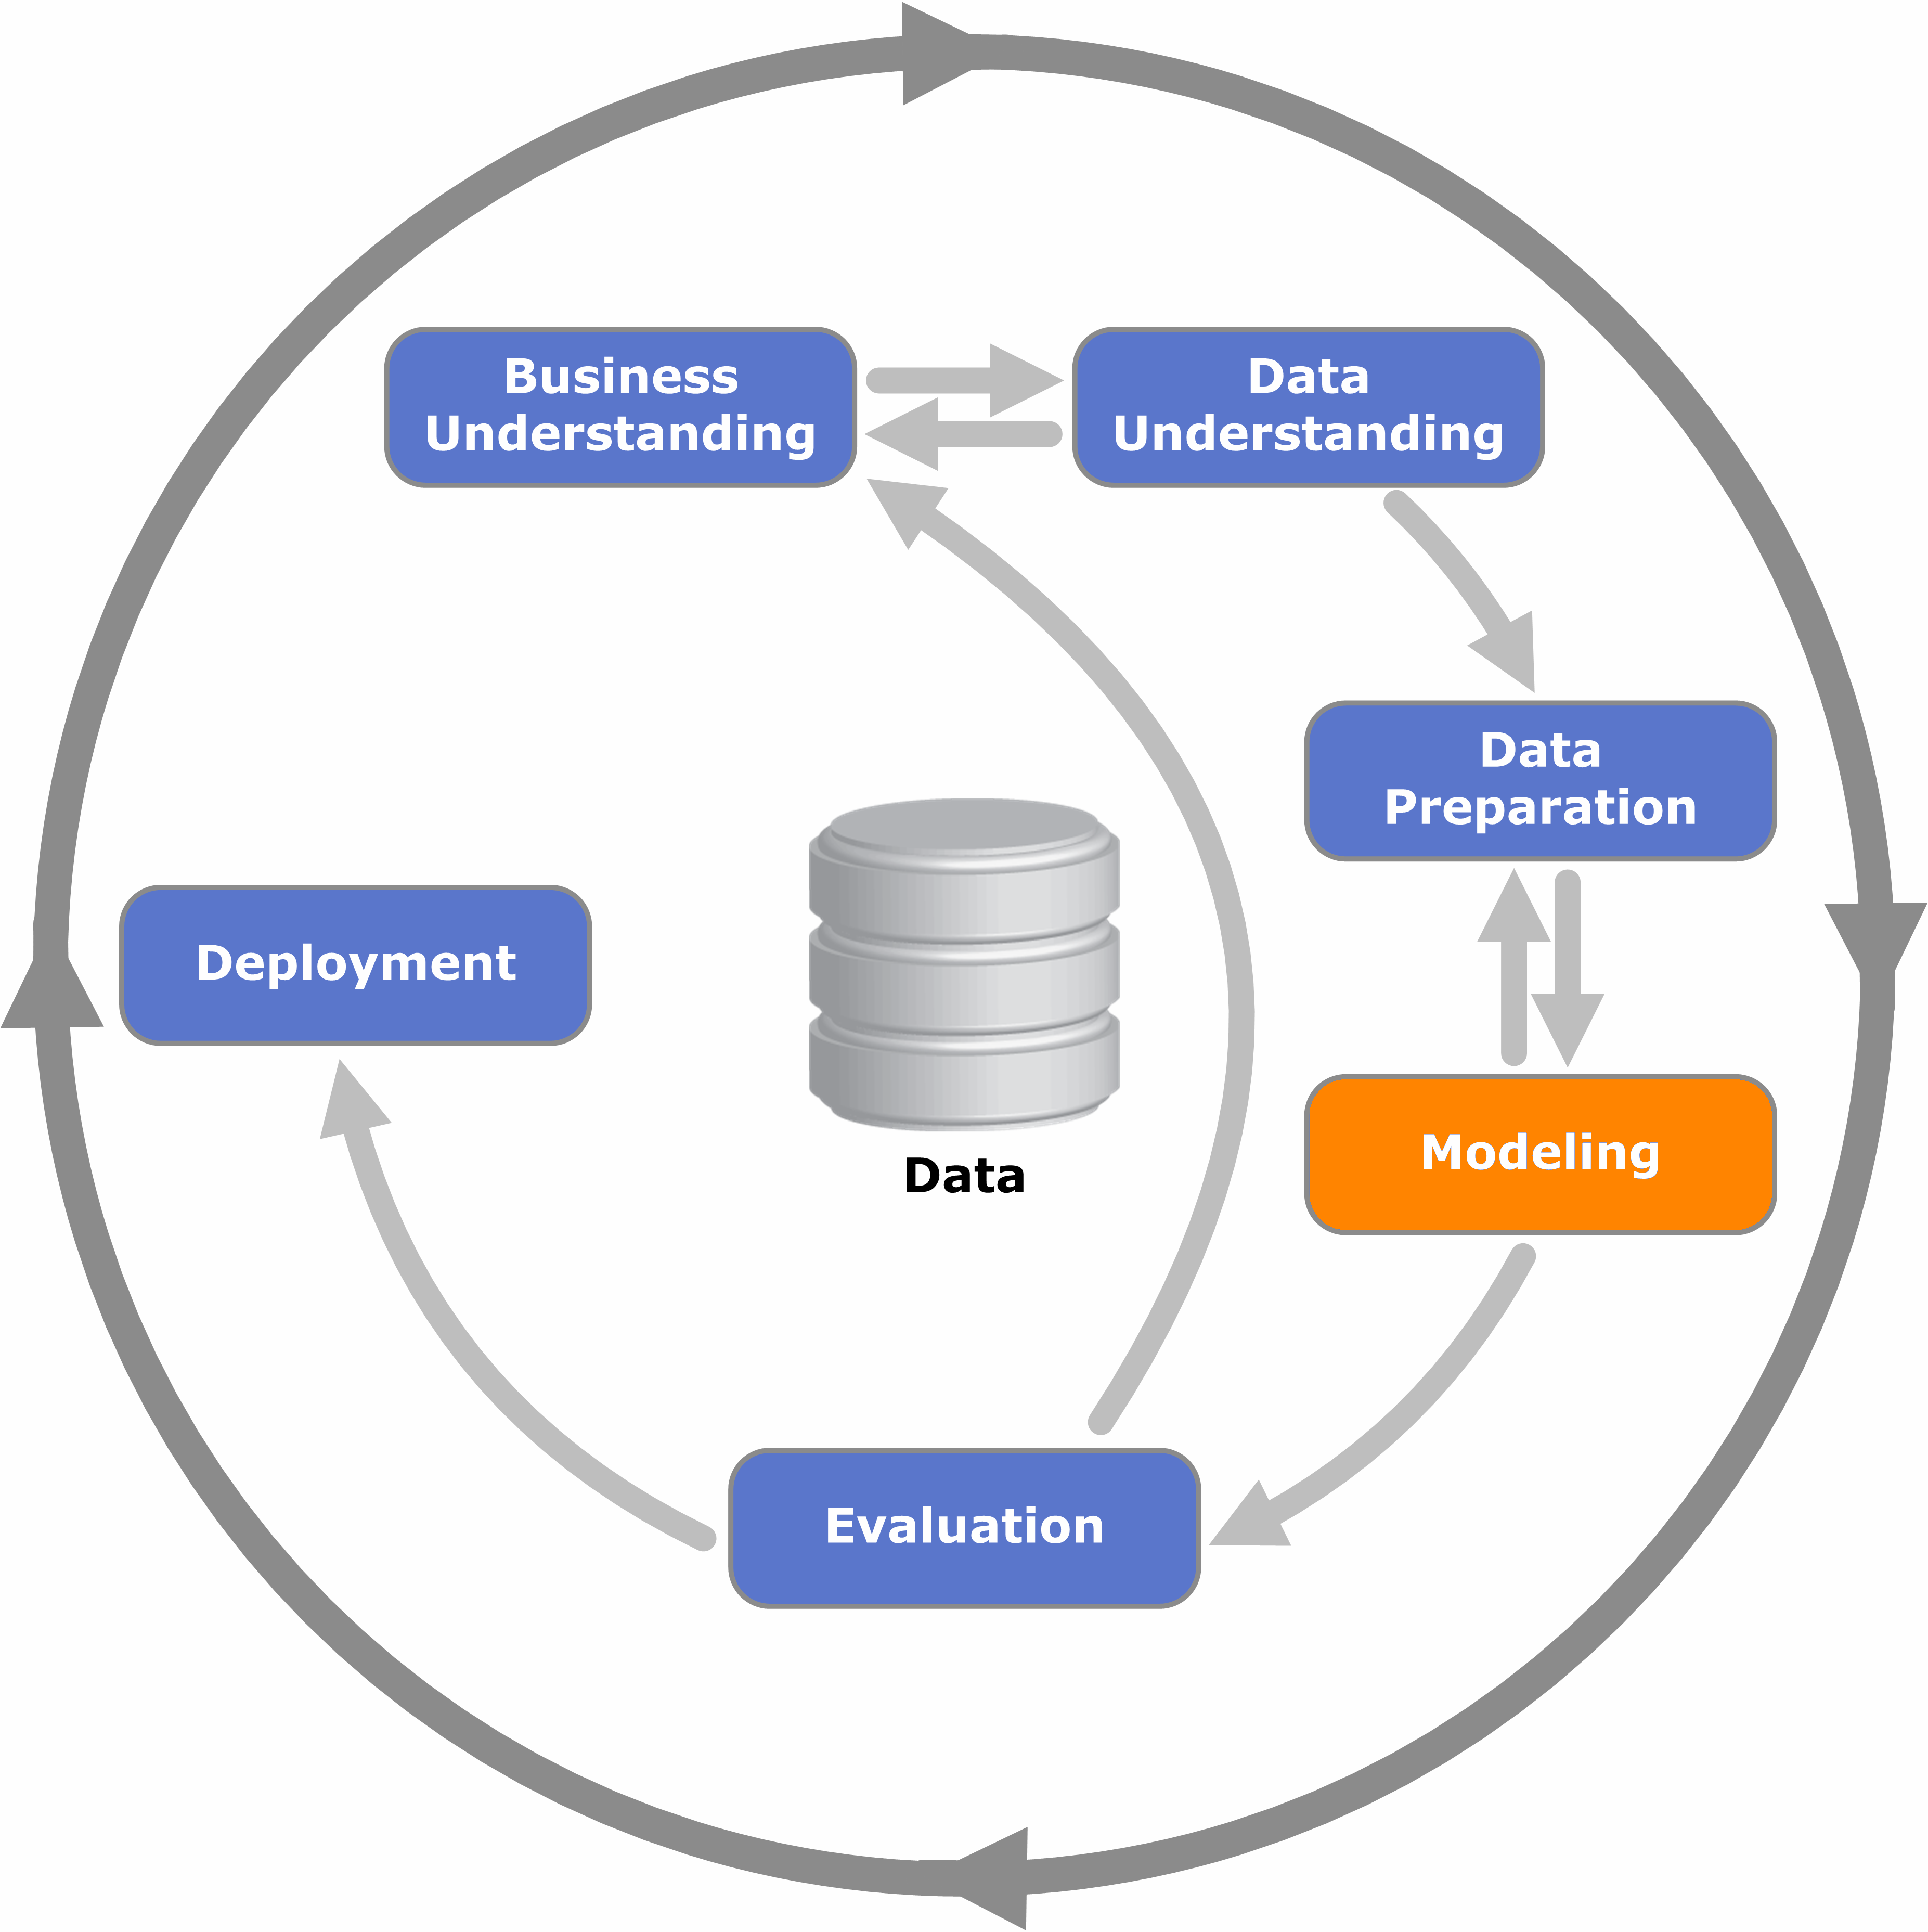
\includegraphics[width=\textwidth]{images/crisp-m.png}
    \end{center}
    \end{column}
  \end{columns}

\end{frame}

\begin{frame}{}

\begin{columns}[C]
    \begin{column}{.5\textwidth}

	\begin{itemize}
	\item точность или аппроксимация?
	\item bias или variance?
	\item интерпретируемость или качество?
	\end{itemize}    
    	
    \end{column}
       
    \begin{column}{.5\textwidth}
    \vspace{-0em}
	\begin{center}
   		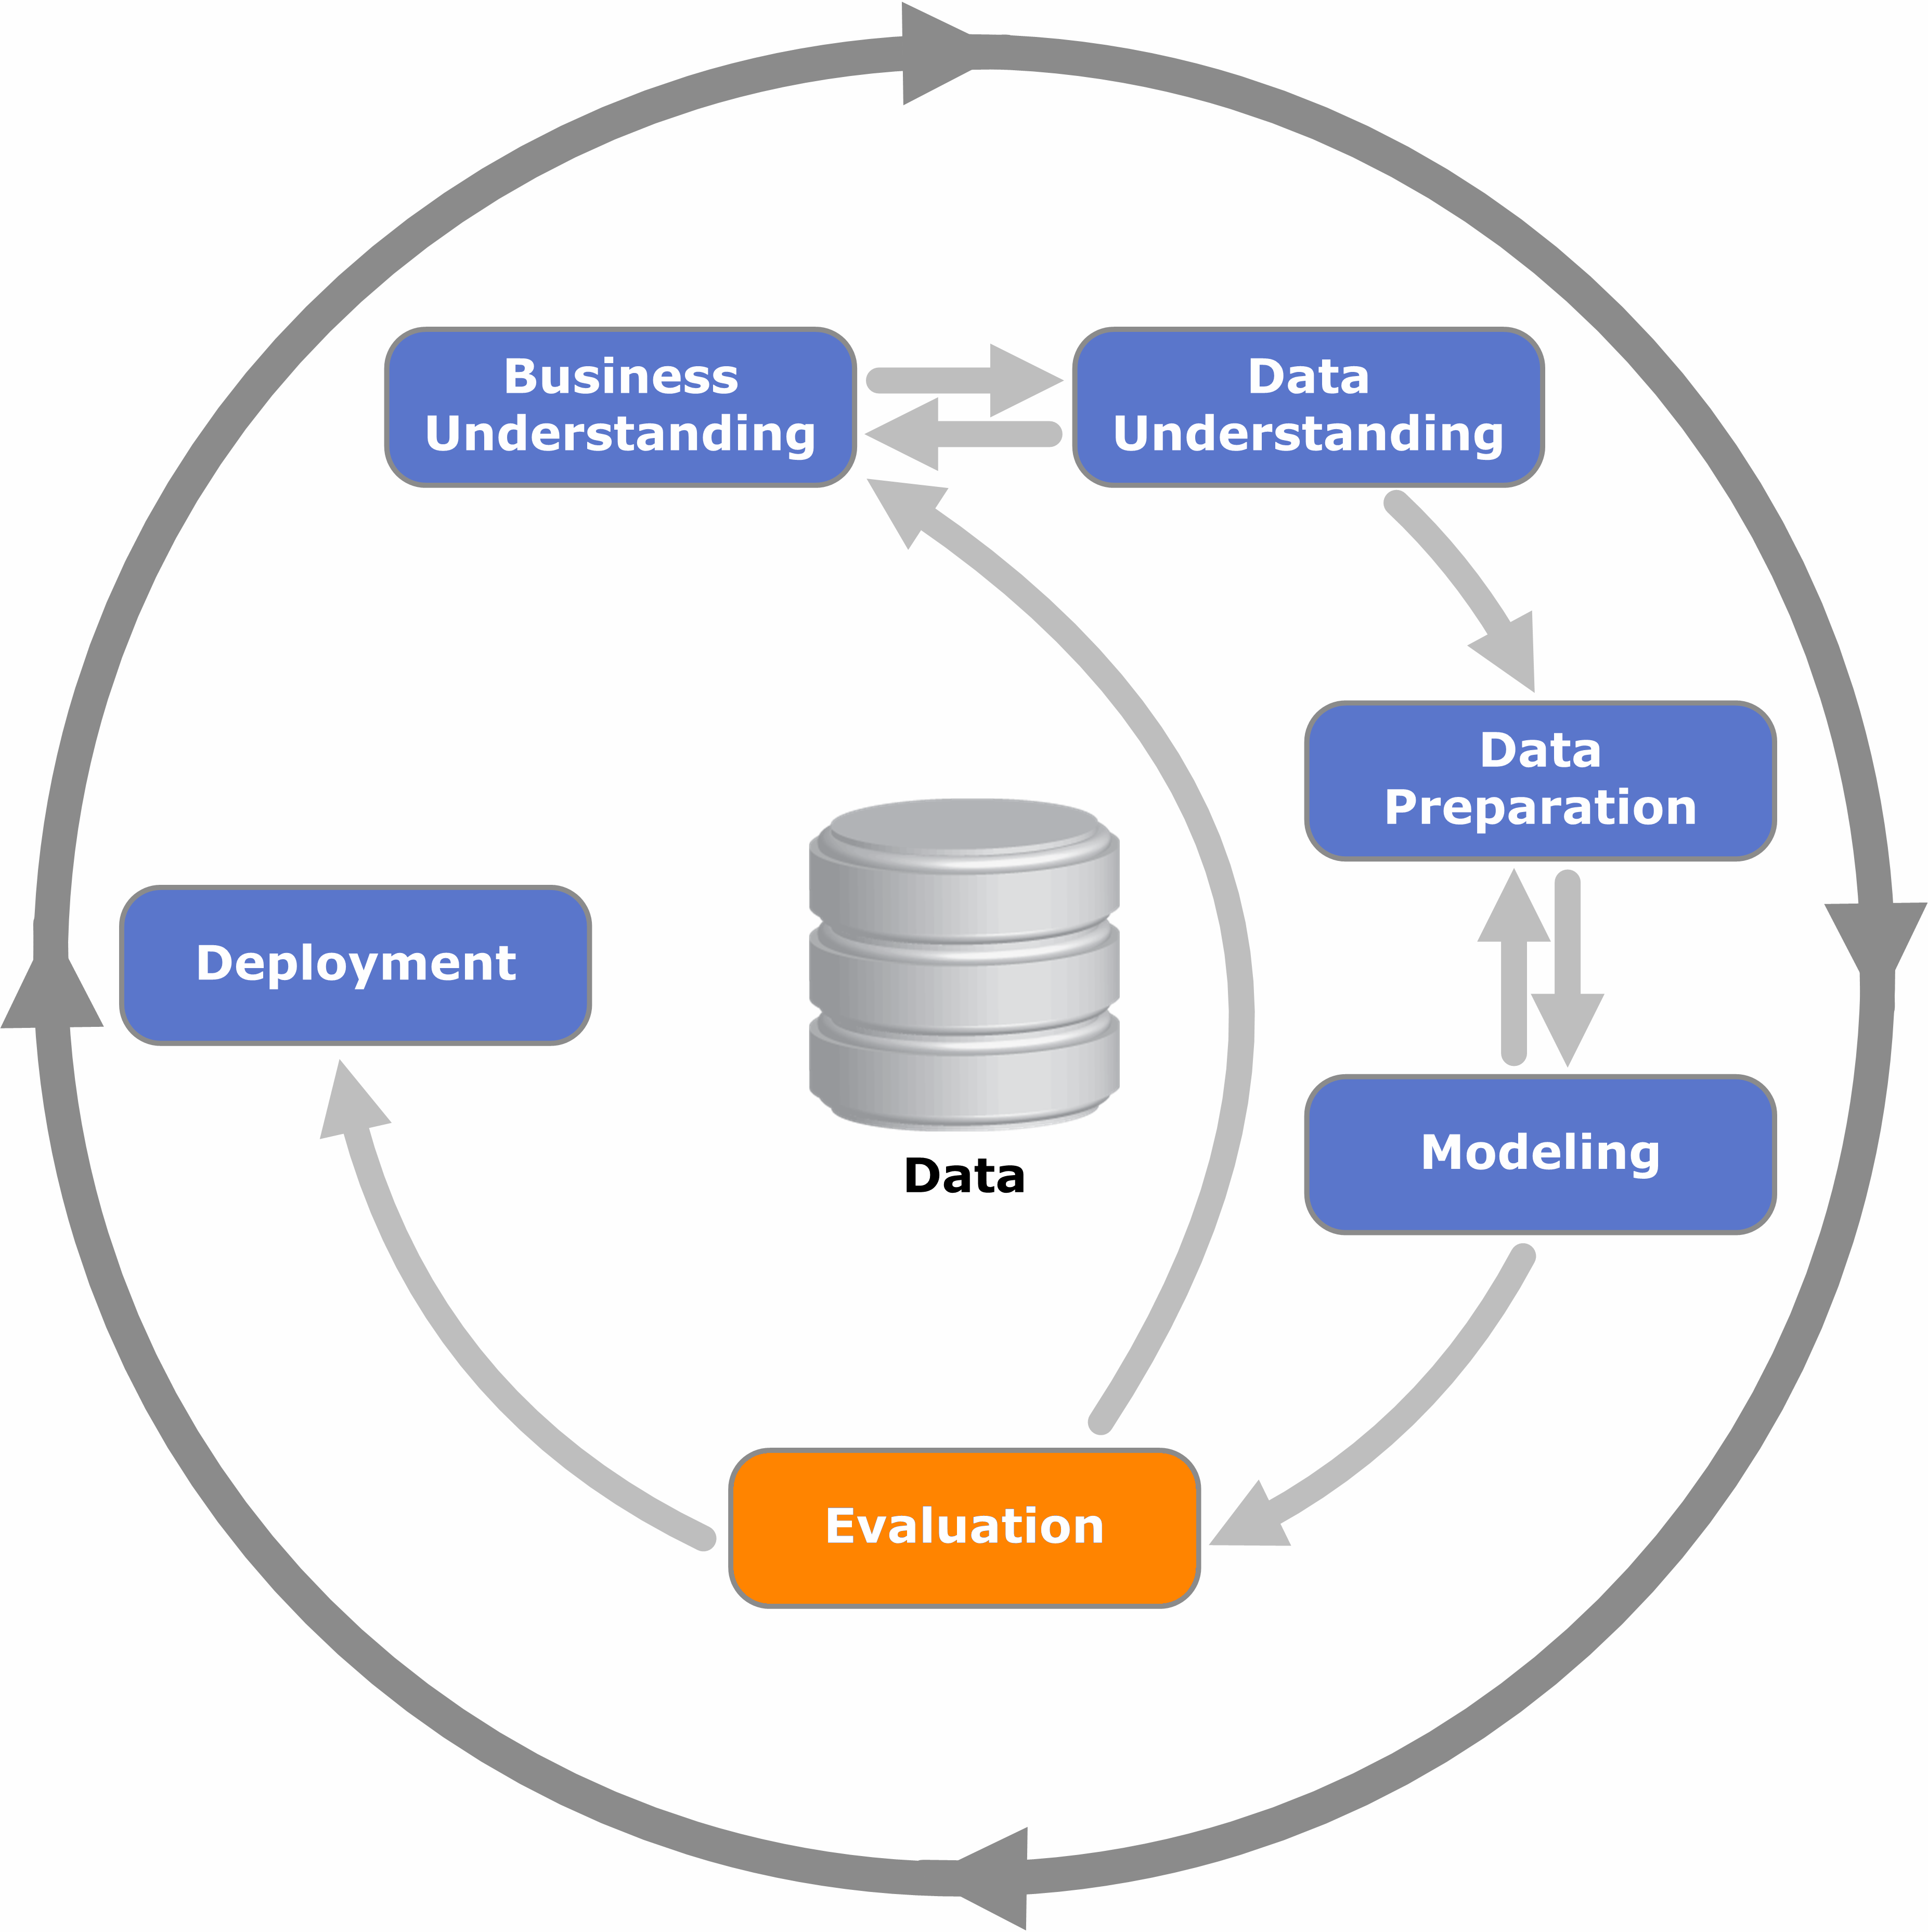
\includegraphics[width=\textwidth]{images/crisp-e.png}
    \end{center}
    \end{column}
  \end{columns}

\end{frame}

\begin{frame}{}

\begin{columns}[C]
    \begin{column}{.5\textwidth}
    	
    \end{column}
       
    \begin{column}{.5\textwidth}
    \vspace{-0em}
	\begin{center}
   		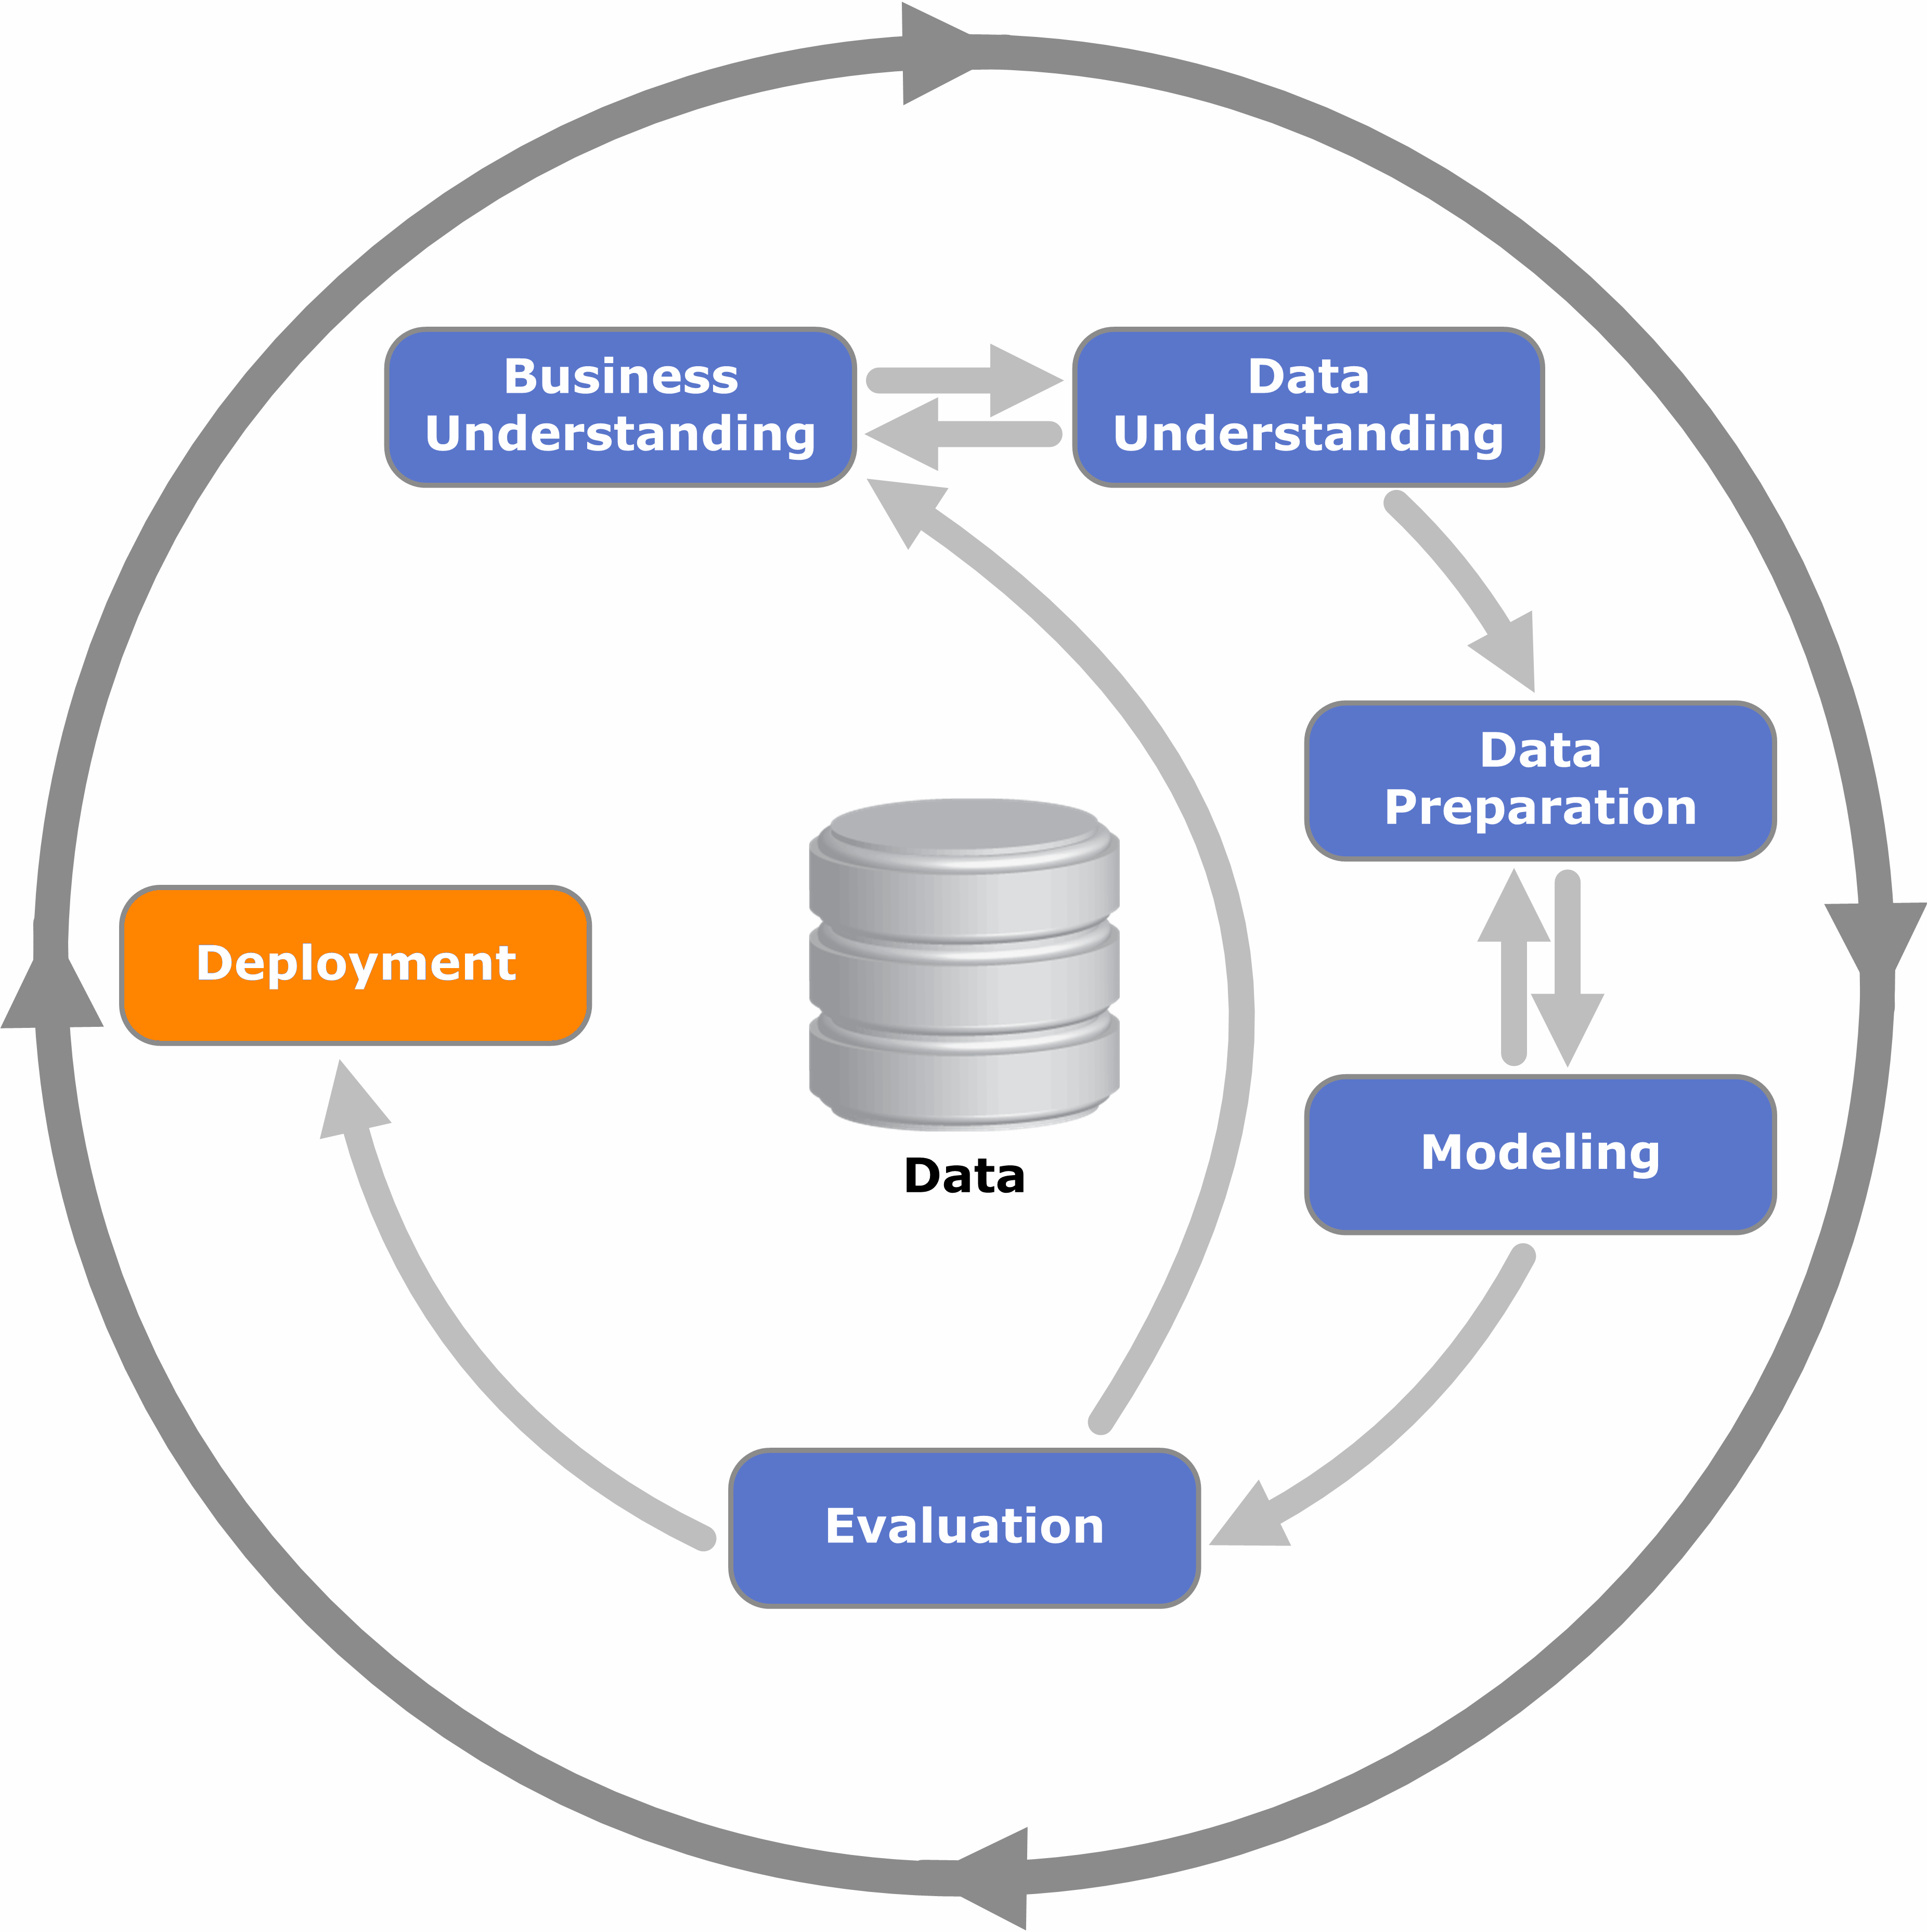
\includegraphics[width=\textwidth]{images/crisp-d.png}
    \end{center}
    \end{column}
  \end{columns}

\end{frame}

% =======================
\section{Exploratory data analysis}
% =======================

\begin{frame}{Exploratory data analysis}

EDA направлен на предварительное изучение данных
\begin{itemize}
\item формироваие гипотез относително структуры данных
\item выбор необходимых инструментов анализа
\end{itemize}
Особенность метода состоит в визуализации и поиске важных характеристик и тенденций

\end{frame}

\begin{frame}{Примеры}

\begin{figure}
        \centering
        \begin{subfigure}[b]{0.3\textwidth}
                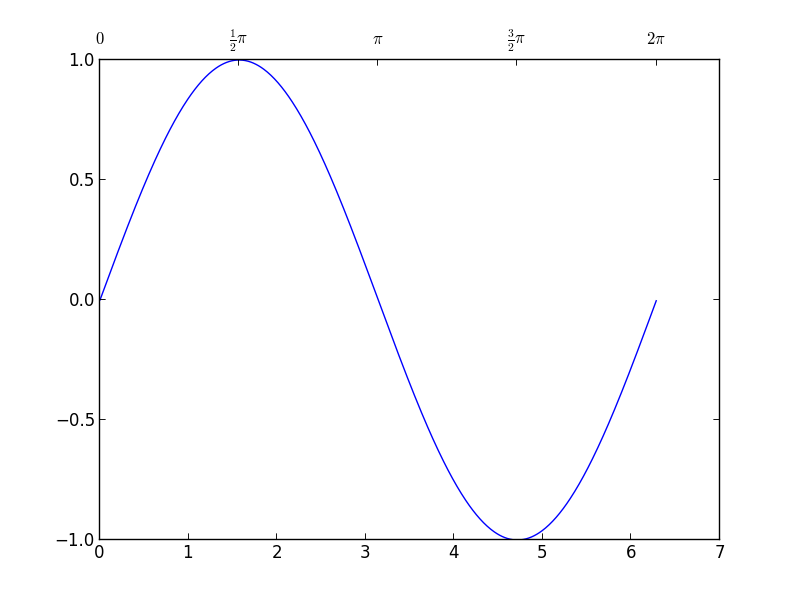
\includegraphics[width=\textwidth]{images/plot.png}
                \caption{Plot}                
        \end{subfigure}%        
        \begin{subfigure}[b]{0.3\textwidth}
                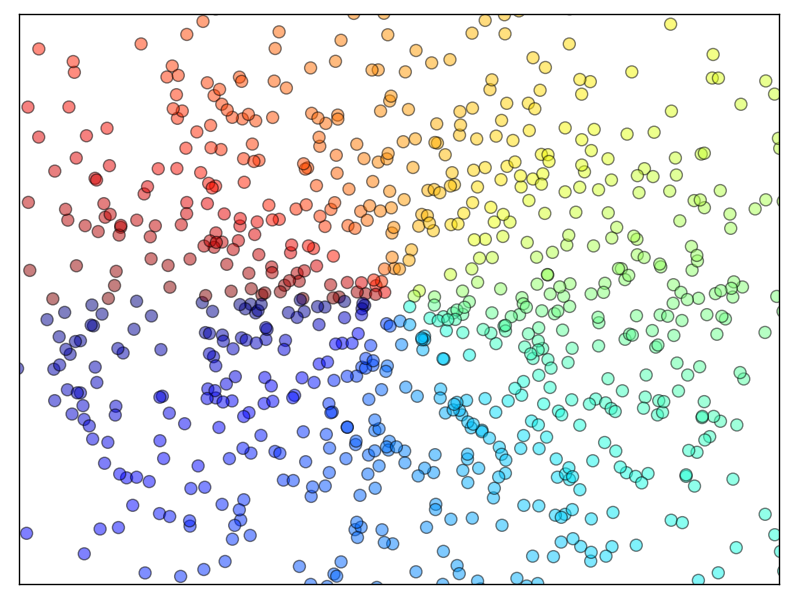
\includegraphics[width=\textwidth]{images/scatter.png}
                \caption{Scatter}     
        \end{subfigure}
        \begin{subfigure}[b]{0.3\textwidth}
                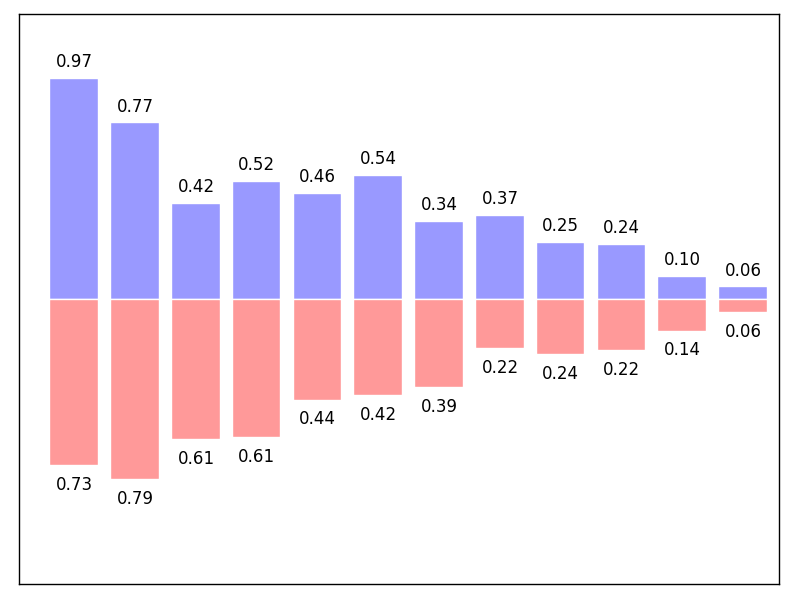
\includegraphics[width=\textwidth]{images/bar.png}
                \caption{Barplot}     
        \end{subfigure}
        
        \begin{subfigure}[b]{0.3\textwidth}
                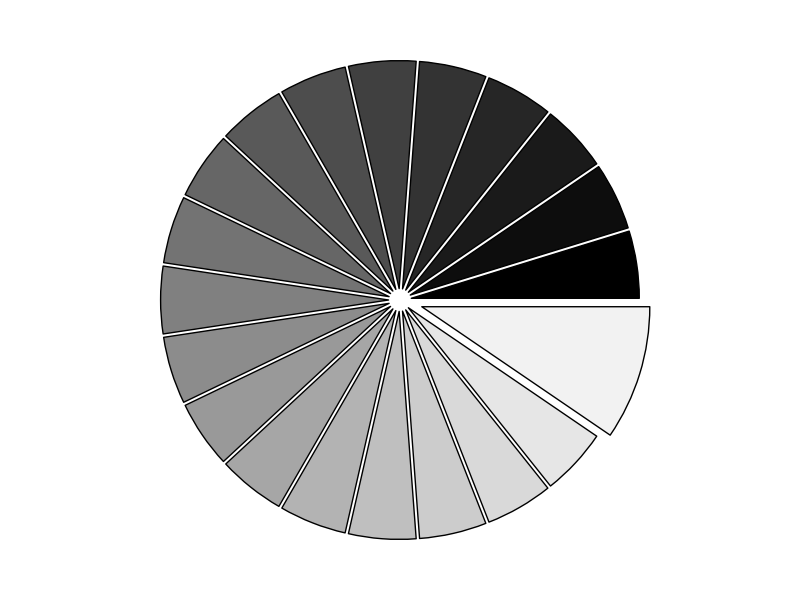
\includegraphics[width=\textwidth]{images/pie.png}
                \caption{Piechart}                
        \end{subfigure}%        
        \begin{subfigure}[b]{0.3\textwidth}
                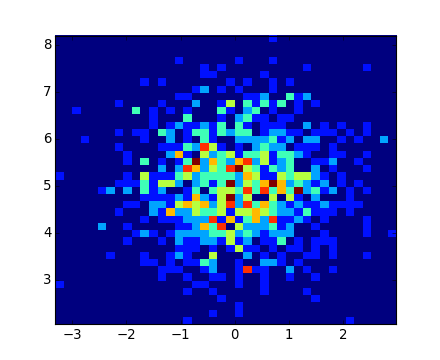
\includegraphics[width=\textwidth]{images/heatmap.png}
                \caption{Heatmap}     
        \end{subfigure}
        \begin{subfigure}[b]{0.3\textwidth}
                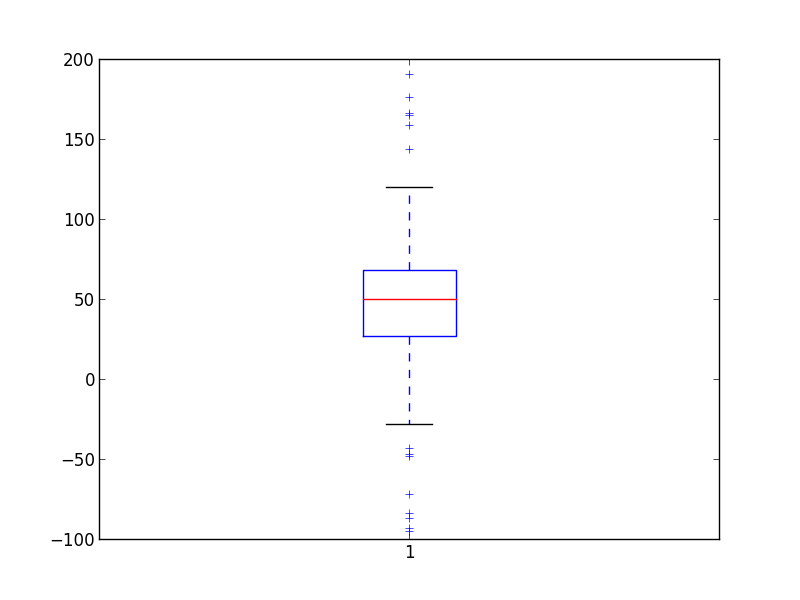
\includegraphics[width=\textwidth]{images/box.png}
                \caption{Boxplot}     
        \end{subfigure}
\end{figure}

\end{frame}

\begin{frame}{Полезные советы}

\begin{columns}[T]
    \begin{column}{.5\textwidth}    	
    	\begin{itemize}
		\item Все познается в сравнении
		\item Причинно-следственные связи
		\item Размерность имеет значение (больше-лучше)
		\end{itemize}	
    \end{column}
    %   
    \begin{column}{.5\textwidth}
    \begin{itemize}
		\item Не избегать пояснений
		\item Content is king
		\end{itemize}		
    \end{column}
  \end{columns}
  
  \begin{center}
   		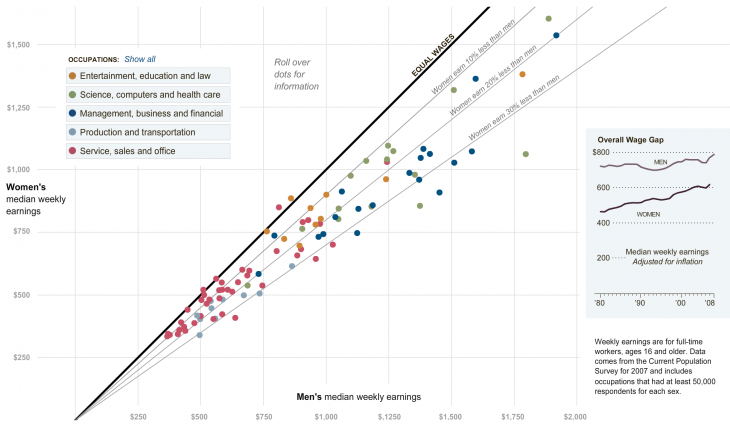
\includegraphics[width=0.8\textwidth]{images/salaries.png}
    \end{center}

\end{frame}

\begin{frame}[fragile]{Задача}

{\bf Дано:} информация о посещении пользователями интернет-сайтов \\
{\bf Требуется:} исследовать распределение количества уникальных пользователей в зависимости от популярности сайта

\vspace{1em}
Пошаговая инструкция
\begin{enumerate}
\item Скачать файл с данными (400M) \url{http://bit.ly/1xdOrHD}
\item Скачать и запустить шаблон кода на python \url{http://bit.ly/1B6fEcO}
\begin{shaded}
{\color{green} \begin{verbatim}
$ python eda.py -h
$ python eda.py -n 20 eda.dat
\end{verbatim}}
\end{shaded}
\item Заполнить функцию \textsf{top\_domain\_user\_counts}
\item Заполнить функцию \textsf{plot\_log\_top\_domains} и посмотреть на распределение в log-log шкале
\item Заполнить функцию \textsf{plot\_linear\_model}, попутно осознав параметры модели
\item Выписать полученное распределение $n_{users}(rank)$
\end{enumerate}

\end{frame}

\begin{frame}[plain]
\begin{center}
{\Large Вопросы}
\end{center}
\end{frame}

\end{document}